% For compilation piecewise (see projekt.tex), it is necessary to uncomment it and change
% \documentclass[../projekt.tex]{subfiles}
% \begin{document}

\chapter{Introduction}

In the rapidly evolving landscape of technology, the rise of quantum computing offers solutions to complex problems that are challenging or even impossible for classical computers. However, this great computational power also introduces a significant vulnerability. As quantum computing advances, it poses a significant threat to the cryptographic systems driving our digital world.

Blockchain is a technology initially popularized by cryptocurrencies like Bitcoin or Ethereum, but it has found usage in broader applications. However, blockchains strongly rely on various cryptographic principles, which makes them vulnerable to potential threats from quantum computers.

Fortunately, researchers are aware of the quantum threat, and institutions such as the National Institute of Standards and Technology (NIST) are actively working on establishing new standards for secure cryptographic algorithms against both quantum and classical computers.

This work explores the potential of integrating new post-quantum (PQ) algorithms into blockchain technology. The objective is to analyze blockchain components vulnerable to quantum attacks, identify appropriate PQ algorithms, and practically implement them within the blockchain. Additionally, the implemented solution compares the performance of multiple PQ and currently used cryptographic algorithms.

The second chapter provides an overview of key concepts and components of blockchain technology. It covers the structure of blocks, transactions, the purpose of consensus mechanisms, and peer-to-peer networks.

The third chapter discusses the quantum threat to existing cryptographic systems and the newly developed PQ cryptography algorithms. This chapter also includes recommendations from relevant institutions such as NSA or NIST. Furthermore, it thoroughly examines PQ algorithms selected as finalists of the NIST competition.

The fourth chapter delves into the specific components of a blockchain that are vulnerable to quantum threats. It explores solutions implemented by existing blockchains that claim to be quantum-resistant and analyzes appropriate PQ cryptography for inclusion in blockchains.

The fifth chapter outlines my design of a PQ blockchain, using PQ cryptography and securing all vulnerable components analyzed in the previous chapter.

Finally, the sixth and seventh chapter provides a detailed overview of the implementation and testing of the designed solution.


%%%%%%%%%%%%%%%%%%%%%%%%%%%%%%%%%%%%%%%%%%%%%%%%%%%%%%%%%%%%%%%%%%%%%%%%%%%%%%
%%%%%%%%%%%%%%%%%%%%%%%%%%%%%%%%%%%%%%%%%%%%%%%%%%%%%%%%%%%%%%%%%%%%%%%%%%%%%%
%%%%%%%%%%%%%%%%%%%%%%%%%%%%%%%%%%%%%%%%%%%%%%%%%%%%%%%%%%%%%%%%%%%%%%%%%%%%%%

\chapter{Blockchain technology}
\label{Blockchain technology}

This chapter serves as a brief introduction to the blockchain technology. It covers the basis of blockchain, how it works, what structures it uses, and what principles it employs.

%%%%%%%%%%%%%%%%%%%%%%%%%%%%%%%%%%%%%%%%%%%%%%%%%%%%%%%%%%%%%%%%%%%%%%%%%%%%%%

\section{Blockchain overview}
\label{sec:Blockchain.overview}

Blockchain is a distributed ledger of cryptographically signed transactions grouped in blocks. These blocks are then linked together so that each block contains a cryptographic hash value of the previous block, as shown in Figure~\ref{figure:bc.chainOfBlocks}~\cite{bc.technology.overview}. The purpose of this design is to ensure the integrity of the blockchain. Even a minor change in any transaction will change the block's cryptographic hash. Since blocks are linked, changes cascade through the subsequent blocks, which makes it easy to detect any alternation. While it is technically possible to recalculate hashes for all blocks, blockchains employ one additional feature preventing such changes. This feature is called a consensus mechanism, and it ensures that changes made to the blockchain require majority agreement among its participants. The consensus mechanism will be discussed later in Section~\ref{Consensus mechanism}.

\begin{figure}[ht]
    \begin{center}
        \scalebox{0.8}{\includegraphics{obrazky-figures/bc-chain.pdf}}
    \end{center}
    \caption{Linked chain of blocks\,--\,blockchain}
    \label{figure:bc.chainOfBlocks}
\end{figure}

From an evolutionary standpoint, a blockchain is characterized as a digital, distributed, decentralized ledger wherein individual participants share and update the ledger within a peer-to-peer (P2P) network according to specific protocols~\cite{vademecun.blockchain}. Figure~\ref{figure:bc.evolution} illustrates the progression from traditional ledgers to blockchain technology. The peer-to-peer (P2P) networks topic will be covered later in Section~\ref{section: P2P}.

\begin{figure}[h]
    \begin{center}
        \scalebox{0.86}{\includegraphics{obrazky-figures/bc-evolution.pdf}}
    \end{center}
    \caption{Evolution from traditional ledger to blockchain \cite{vademecun.blockchain}}
    \label{figure:bc.evolution}
\end{figure}

Blockchain technology contains its own key features such as~\cite{comprehensive.survey.blockchain}:
\begin{itemize}
    \item \textbf{Security}\,--\,transactions must be cryptographically signed to prevent falsification and blockchain changes must be validated by the majority of participants or validators.
    \item \textbf{Transparency}\,--\,transaction history is available to all blockchain participants.
    \item \textbf{Decentralization}\,--\,there is no central authority controlling the validation of the transactions.
    \item \textbf{Immutability}\,--\,once the transaction has been validated and inserted into a blockchain, it is impossible to change or remove it.
    \item \textbf{Programmability}\,--\,ability to execute smart contracts.
\end{itemize}

Furthermore, blockchains do not depend on centralized trusted authorities to process transactions. Also, there is no need for third-party verification and validation of the transactions~\cite{comprehensive.survey.blockchain}. Verification and validation in blockchain are accomplished through mutual confirmation of transactions and consensus among participants in the network. Not all of these features are always applied to every blockchain. As will be discussed further in Section~\ref{Blockchain classification}, different types of blockchain may have other purposes so that they may use just some of the mentioned features.

Blockchain technology became popular mainly because of the popular cryptocurrency Bitcoin, which idea was described by Satoshi Nakamoto in the original paper~\cite{nakamoto2009bitcoin} from 2008. Nakamoto's paper presents an important idea and possible solutions for a decentralized payment system. Bitcoin as a cryptocurrency was created later in 2009 based on this idea. It is important to note that blockchain is not synonymous with cryptocurrency. While blockchain is the underlying technology for many cryptocurrencies, its applications extend beyond payments or currencies. For example, blockchains can be used for storing electronic medical records, digital certificates, tracking supply chain management, voting systems, and many other applications. 

However, despite its unique features and popularity, blockchain technology is not suitable in all cases. Belotti et al. in~\cite{vademecun.blockchain} delve into the considerations for determining the suitability of blockchain for specific purposes. It includes a straightforward decision map that shows whether it is appropriate to use blockchain or traditional ledger technology.

%%%%%%%%%%%%%%%%%%%%%%%%%%%%%%%%%%%%%%%%%%%%%%%%%%%%%%%%%%%%%%%%%%%%%%%%%%%%%%

\section{Blockchain classification}
\label{Blockchain classification}

There are two main classifications of blockchains based on access control: permission-less and permissioned blockchains~\cite{comprehensive.survey.blockchain}.

\subsection{Permission-less blockchain}

A Permission-less blockchain network is accessible to anyone who wants to join the blockchain\hyphenation{block-chain} network. Anyone can publish a new block or create/read the transactions on the blockchain. Furthermore, there are no specialized nodes with any privileged rights. Because anyone can publish a new block, there has to be a mechanism that prevents malicious users from publishing blocks in a way that subverts the system. For this reason, an essential part of the permission-less blockchain is a consensus mechanism. An example of such a blockchain is a \textbf{public blockchain}. Well-known public blockchains are, for example, Bitcoin or Ethereum~\cite{bc.technology.overview}.

\subsection{Permissioned blockchain}

A permissioned blockchain network is accessible only with permission from some authority. Since only authorized nodes maintain the blockchain, it is possible to restrict read access, who can issue transactions, and who can publish a block. Additionally, it increases the level of trust in a blockchain. Permissioned blockchain also uses a consensus algorithm, but these methods often do not require as significant resources as in the case of permission-less blockchains~\cite{bc.technology.overview}. Permissioned blockchain can be further divided into three categories: \textbf{private blockchain}, \textbf{consortium blockchain}, and \textbf{hybrid blockchain}. 

\subsubsection{Private blockchain}

A private blockchain is a type of permissioned blockchain suitable, for example, for a~smaller company. It can bring scalability because it does not influence speed and efficiency even if the network grows. Moreover, in case of any mishap, it is easy to identify the nodes involved in the transactions. The main disadvantage is that the whole blockchain is controlled by the organization as a centralized unit~\cite{comprehensive.survey.blockchain}. In addition, data on the blockchain has great redundancy. Each node on the blockchain can own a copy of the data which can serve as a~backup. Well-known private blockchains are, for example, Hyperledger Fabric or Ethereum Enterprise.

\subsubsection{Consortium blockchain}

A consortium blockchain is similar to a private blockchain, but it is managed by multiple organizations. It incorporates features from both private and public blockchains. Some important aspects of the organizations could be private, while others can remain public~\cite{comprehensive.survey.blockchain}. Well-known consortium blockchains are, for example, Quorum or R3 Corda.

\subsubsection{Hybrid blockchain}

A hybrid blockchain takes the best from private and public blockchains. The consensus mechanism can be optimized since only a few nodes are authorized to validate the transaction~\cite{comprehensive.survey.blockchain}. As an example, it can serve the Dragonchain blockchain.

\begin{figure}[h]
    \begin{center}
        \scalebox{1}{\includegraphics{obrazky-figures/bc-classification.pdf}}
    \end{center}
    \caption{Classification of blockchains~\cite{comprehensive.survey.blockchain}}
    \label{figure:bc.typesTree}
\end{figure}


%%%%%%%%%%%%%%%%%%%%%%%%%%%%%%%%%%%%%%%%%%%%%%%%%%%%%%%%%%%%%%%%%%%%%%%%%%%%%%

\section{Blocks}
\label{bc block}

A blockchain block is a data structure composed of transactions (data) and a header. The header contains metadata designed to identify the block and enable the verification of its content.

Each implementation of a blockchain can define its own block structure. However, some data fields are frequently utilized by the majority of them~\cite{bc.technology.overview}:

\bigskip

\begin{itemize}
    \item \textbf{Block Header}
    \begin{itemize}
        \item The block number, also known as block height or sequence number. It is a unique identifier of the block.
        \item Hash value of the previous block
        \item A hash representation of the block data. It can be a hash of all the combined block data, or a common practice is to generate a Merkle tree and store the root hash there (more about Merkle trees is discussed further in this section).
        \item A timestamp
        \item The size of the block
    \end{itemize}
    Blockchains utilizing the Proof-of-Work (PoW) consensus mechanism can also include a nonce value field. It is a number manipulated by the publishing node to solve the PoW puzzle. 
    \item \textbf{Block Data}
    \begin{itemize}
        \item A list of validated transactions and ledger events included within the block
        \item Other data may be present (account balances etc.)
    \end{itemize}
\end{itemize}


\begin{figure}[h]
    \begin{center}
        \scalebox{1.1}{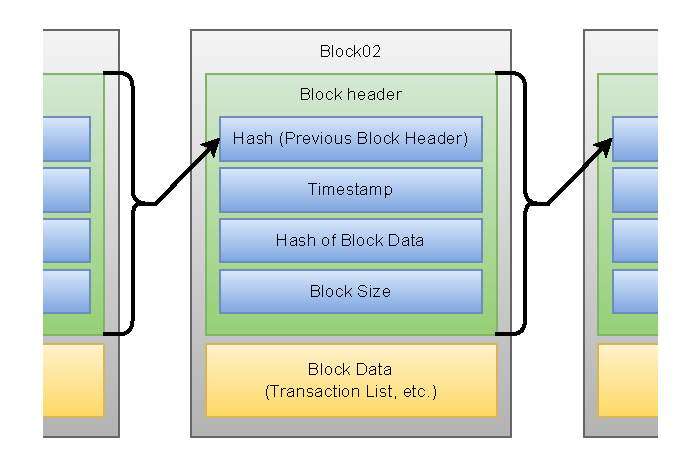
\includegraphics{obrazky-figures/bc-blocks.pdf}}
    \end{center}
    \caption{Generic Chain of Blocks \cite{bc.technology.overview}}
    \label{figure:bc.block}
\end{figure}


\subsubsection{Merkle trees}
\label{Merkle trees}

Merkle tree (patented in 1989~\cite{merkle.tree.patent}) is a hash tree procedure that consists of data (transactions) that are iteratively hashed in pairs~\cite{vademecun.blockchain}. The transactions, represented as leaf nodes, are hashed, and then every two hashes are put in a pair and hashed again until everything is hashed in one root hash. If the number of transactions is odd, the last transaction is duplicated and hashed with itself. The example of a Merkle tree is shown in Figure~\ref{figure:bc.merkle tree}.

The primary purpose of the Merkle tree root hash in a block header is to easily verify the integrity of the transaction in the block.

\begin{figure}[ht]
    \begin{center}
        \scalebox{0.76}{\includegraphics{obrazky-figures/merkle-tree.pdf}}
    \end{center}
    \caption{Merkle hash tree with transactions $T_0$-$T_9$.}
    \label{figure:bc.merkle tree}
\end{figure}


%%%%%%%%%%%%%%%%%%%%%%%%%%%%%%%%%%%%%%%%%%%%%%%%%%%%%%%%%%%%%%%%%%%%%%%%%%%%%%

\section{Transactions}
\label{Transactions}

Transactions come into place whenever users want to interact with one another in the blockchain network. Transactions do not have to be strictly financial and do not just carry and store transaction data. Different blockchain implementations can implement their own structure of transactions and the way transactions are performed. The usage of blockchain transactions is not limited, for example, a transaction can be a piece of code that will be executed after certain circumstances are met, this is also called a smart contract~\cite{vademecun.blockchain}.

\bigskip

\noindent The journey of a transaction (also illustrated in Figure~\ref{figure:bc.transaction})~\cite{vademecun.blockchain}:

\begin{itemize}
    \item \emph{Creation:} The transaction's sender defines, according to blockchain transaction structure, the digital asset's source and destination.
    \item \emph{Propagation:} The transaction is propagated through leading nodes\footnote{Nodes that are distributing transactions, blocks, and other blockchain messages} to validating nodes in a Peer-to-Peer (P2P) network.
    \item \emph{Validation:} During this stage, transactions, organized into blocks, must successfully navigate the various phases of the envisioned consensus mechanism to be considered valid and, consequently, executable. Afterward, the block with transactions can be attached as the next block to the blockchain.
    \item \emph{Propagation:} The block with the transaction is propagated through the blockchain network to let all nodes update their copy of the blockchain.
    \item \emph{Confirmation:} The transaction is executed only if the block with transactions is validated and eventually published on the blockchain. If there are two valid chains, nodes must agree on a single chain of blocks (this is also the function of the consensus mechanism). Once confirmed, this block will become an immutable part of the final ledger version and may no longer be discarded.
\end{itemize}


\begin{figure}[h]
    \begin{center}
        \scalebox{0.83}{\includegraphics{obrazky-figures/tx-journey.pdf}}
    \end{center}
    \caption{The Transaction Journey~\cite{vademecun.blockchain}}
    \label{figure:bc.transaction}
\end{figure}

It is crucial to note transactions are critically dependent on cryptography. Each transaction requires a unique sender signature to prevent falsification and ensure integrity. If a~transaction is altered or includes an invalid signature, it is rejected. Figure~\ref{figure:digital.signature} shows how digital signature is performed. It is essential to securely store the private (secret) key to prevent potential attackers from gaining access. If the private key is stolen, an attacker could exploit the opportunity to sign transactions.

\begin{figure}[h]
    \begin{center}
        \scalebox{0.94}{\includegraphics{obrazky-figures/tx-signature.pdf}}
    \end{center}
    \caption{Example of signing a transaction}
    \label{figure:digital.signature}
\end{figure}

Another challenge that blockchain addresses is double-spending. In transactions involving electronic assets, the blockchain must verify that the sender is the legitimate owner of the asset. To guarantee ownership, the blockchain maintains a record of asset ownership. This is commonly addressed through data models like UTXO, Account, UTXO$^+$, or Key-value.


%%%%%%%%%%%%%%%%%%%%%%%%%%%%%%%%%%%%%%%%%%%%%%%%%%%%%%%%%%%%%%%%%%%%%%%%%%%%%%

\section{Peer-to-peer network}
\label{section: P2P}

Peer-to-peer (P2P) networks are interconnected collections of nodes, which communicate together. Participants in P2P are known as peers. The main benefit of using the P2P network is file/data sharing. In centralized systems, the download mainly depends on the strength of the server, while in the decentralized P2P network, if one of the peers fails to operate, the other peers in the network can finish the required action~\cite{comprehensive.survey.blockchain}. The difference between centralized and decentralized (P2P) network is illustrated in Figure~\ref{figure:p2p-network}.

Blockchains utilize a P2P network to maintain decentralization. There is no central server functioning as an intermediary to process transactions; instead, transactions are distributed among nodes within the blockchain.

\begin{figure}[h]
    \begin{center}
        \scalebox{0.8}{\includegraphics{obrazky-figures/p2p-network.pdf}}
    \end{center}
    \caption{Comparison of centralized and P2P network}
    \label{figure:p2p-network}
\end{figure}

%%%%%%%%%%%%%%%%%%%%%%%%%%%%%%%%%%%%%%%%%%%%%%%%%%%%%%%%%%%%%%%%%%%%%%%%%%%%%%

\section{Consensus mechanism}
\label{Consensus mechanism}

Since there is no trusted third party or central authority a consensus mechanism is an algorithm based on predefined rules that determines the node that publishes the next block or ensures that nodes cooperate to create the next block. To add a new block to the blockchain, all nodes must reach a common agreement over time. In permission-less blockchains publishing nodes usually compete to publish the next block. They do this to get revenue through cryptocurrency or transaction fees. In permissioned blockchains, a consensus can be reached more easily because of the trust between nodes~\cite{bc.technology.overview}. Nodes responsible for reaching consensus are called validators; in the case of the Proof-of-Work (PoW) consensus mechanism, they can be called miners.

The consensus mechanism also solves situations when different nodes publish a block at approximately the same time. This event is also called a fork. The example of a blockchain fork is shown in Figure~\ref{figure:bc.valid.chain}. In most of the blockchain networks is "longer" chain viewed as the correct one. The other chains will be considered invalid and discarded~\cite{bc.technology.overview}.
This mechanism relies on the assumption that the majority of nodes in the blockchain are honest so they always create longer chains than malicious ones.

A scenario in which a fork may occur is when a malicious node publishes a block containing invalidated transactions that were not propagated. If the malicious node eventually wins in the competition and publishes this block on the blockchain, other nodes with a~different block will persist in trying to publish their own block, leading to the creation of two branches. One of these branches includes the block with invalid transactions. While the malicious node continues to compute new blocks on its branch, other nodes on the blockchain persist in working on the correct branch. Over time, the correct branch will naturally become longer and be chosen as the correct chain.

\begin{figure}[h]
    \begin{center}
        \scalebox{1.1}{\includegraphics{obrazky-figures/bc-fork.pdf}}
    \end{center}
    \caption{Example of a blockchain valid nodes}
    \label{figure:bc.valid.chain}
\end{figure}

There are many types of consensus mechanisms. Each blockchain can implement its own to exactly meet its needs and purpose. The widely used consensus mechanisms are Proof-of-Work (PoW) and Proof-of-Stake (PoS), which are described more in detail below, but there are many others like Proof of Burn (PoB), Proof of Capacity (PoC), Proof of Space (PoSpace), and others. The final consensus mechanism among the three outlined below is the XRP consensus mechanism. It claims more detailed exploration, as it is chosen for utilization in subsequent design and implementation.

\subsubsection{Proof-of-Work (PoW)}

The proof-of-work consensus mechanism operates on the principle of solving a computationally intensive puzzle. Nodes engaging in the solution of this puzzle are commonly referred to as miners or miner nodes. The successful solution of the puzzle serves as "proof" that they have expended computational effort. It is based on the concept that computing the puzzle is hard, but verifying is easy~\cite{bc.technology.overview}.

As an illustration, a common method involves determining a nonce value for the block. The nonce is a value that, when hashed with the block's hash, produces a hash containing a specific number of leading zeros. The computational challenge lies in finding this nonce, which requires extensive trial and error. Conversely, the verification process is simple, it requires to calculate just one hash~\cite{bc.technology.overview}.

A notable drawback of the PoW consensus mechanism is its demand for computational power, which can lead to significant electricity consumption. This characteristic raises concerns about its environmental sustainability, as the energy-intensive character of the process is not aligned with eco-friendly practices.

\subsubsection{Proof-of-Stake (PoS)}

The proof-of-stake consensus mechanism is based on an election of the validator that validates the next block. Participation in the validator election requires the possession of a~stake, denoting a certain amount of cryptocurrency. A higher stake means a higher probability of being elected as the next validator. This is far less computationally intensive than PoW, but it concentrates the validation among the wealthiest nodes. On the other hand, the wealthier nodes may have a vested interest in accurate validation~\cite{vademecun.blockchain}.

\subsubsection{XRP Ledger Consensus Protocol}

XRP Ledger Consensus Protocol is a type of Federated Byzantine Agreement consensus mechanism. It consists of a special type of nodes called \emph{validators} that are trusted by other nodes. Each participant on the network creates a unique node list (UNL) of chosen validator nodes. This list is in full competence of each node so each node can choose other nodes it trusts. The philosophy behind this is that nodes gravitate toward reliable validators, while nonreliable validators have a smaller impact.

Validators receive candidate transactions and proposals. Candidate transactions are transactions seeking inclusion in the next version of the ledger\footnote{In the case of XRP a ledger is something like a block. It represents a new blockchain state.}. Proposals are a special kind of message between validators. It contains a set of transactions that a validator proposes to other validators. Validators communicate and update proposals until a supermajority of chosen validators agree on the same set of transactions. Consensus is an iterative process. At the start of the first round, at least 50\% of validators must agree. In subsequent rounds, this threshold is increasing up to 80\%. Candidate transactions not included in the agreed-upon proposal remain candidate transactions and may be considered again in the next version of the ledger. This phase is called the \textbf{deliberation} phase~\cite{XRP.analysis,XRP.consensus}.

The next phase is called \textbf{validation}. In this phase, nodes decide whether to fully validate a ledger based on the validations issued by trusted nodes. It can be broken up into two parts~\cite{XRP.analysis,XRP.consensus}:
\begin{itemize}
    \item Calculating the resulting ledger version from an agreed-upon transaction set.
    \item Comparing results and declaring the ledger version validated if enough trusted validators agree.
\end{itemize}

If the network fails to achieve supermajority agreement on validations, it stops making further progress, and the consensus mechanism is repeated. Over time, there is an increasing likelihood that a majority of the validators within the network have received an identical set of candidate transactions. This ensures that each consensus round decreases disagreement among the validators~\cite{XRP.analysis,XRP.consensus}.

Notice that XRP consensus is built on a different principle than PoW or PoS. While in PoW and PoS, the next block publisher competes to become the next validator, in XRP, consensus nodes rather cooperate to achieve the consensus.

%%%%%%%%%%%%%%%%%%%%%%%%%%%%%%%%%%%%%%%%%%%%%%%%%%%%%%%%%%%%%%%%%%%%%%%%%%%%%%

\section*{Blockchain technology summary}

To summarize, a blockchain is a distributed, decentralized, immutable ledger of transactions organized into blocks and connected through cryptographic hashes. Fundamental elements of blockchain include asymmetric cryptography, digital signatures, and cryptographic hashes. Communication within the blockchain occurs through a peer-to-peer (P2P) network. The verification and validation of transactions on the blockchain are accomplished through a specific algorithm known as the consensus mechanism.

%%%%%%%%%%%%%%%%%%%%%%%%%%%%%%%%%%%%%%%%%%%%%%%%%%%%%%%%%%%%%%%%%%%%%%%%%%%%%%
%%%%%%%%%%%%%%%%%%%%%%%%%%%%%%%%%%%%%%%%%%%%%%%%%%%%%%%%%%%%%%%%%%%%%%%%%%%%%%
%%%%%%%%%%%%%%%%%%%%%%%%%%%%%%%%%%%%%%%%%%%%%%%%%%%%%%%%%%%%%%%%%%%%%%%%%%%%%%

\chapter{Quantum threat and post-quantum cryptography}
\label{Quantum threat and Post-quantum cryptography}

This chapter discusses the risks posed by quantum computers and the corresponding solutions. A significant concern is their potential to undermine current cryptography. However, there is promising progress in developing new post-quantum (PQ) cryptographic algorithms designed to withstand attacks from quantum computers.

The first Section~\ref{Quantum threat} outlines challenges, threats, and existing solutions in the PQ world. It also provides an overview of the PQ algorithms that will be analyzed in this work. Section~\ref{pq.recommendations} delves into recommendations for PQ cryptography from relevant institutions. Sections~\ref{sec: KEM} and~\ref{sec: signatures} offer a more detailed examination of Key Encapsulation Mechanism (KEM) algorithms and digital signature algorithms, as they are particularly vulnerable to quantum threats. Lastly, Section~\ref{sec:pq.crypto.summary} presents a comprehensive comparison, assessing the sizes of public and private keys, ciphertexts, signatures, and performance of the mentioned PQ algorithms. It concludes with a summary of this chapter and highlights the disparities between currently used cryptography and new PQ cryptography.


%%%%%%%%%%%%%%%%%%%%%%%%%%%%%%%%%%%%%%%%%%%%%%%%%%%%%%%%%%%%%%%%%%%%%%%%%%%%%%

\section{Quantum threat}
\label{Quantum threat}

Quantum computers are a new type of computers that utilize the principles of quantum mechanics. In the future, there are assumptions that quantum computers at some tasks will outperform the current microtransistor-based systems, which are already reaching their limits. Although new technologies bring new opportunities and solutions, they also bring new risks and vulnerabilities if misused. In the case of quantum computers, the risks are mainly associated with threats to the currently used cryptography~\cite{NUKIB.report}.

A specific concern arises from the capability of quantum computers to solve certain mathematical problems much more efficiently than classical computers. Many existing encryption algorithms rely on these mathematical problems' complexity, which makes them vulnerable to quantum threats~\cite{pqc.survey.7030040}.

There are already algorithms designed specifically for quantum computers that pose a~direct threat. Notably, Shor's algorithms~\cite{shore.alg} address the efficient factorization of large numbers and the Discrete Logarithm problem. These problems exhibit exponential complexity on classical computers but only linear complexity on quantum computers. This poses a direct risk to current asymmetric cryptography. Specifically for algorithms RSA and DSA, as well as elliptic curves algorithms Ed25519 or ECDSA. All currently used asymmetric algorithms based on the problem of factoring large numbers and the problem of solving a discrete logarithm can be broken in the future precisely with the use of a quantum computer and Shor's algorithm.

Additionally, Grover's algorithm~\cite{grover.alg}, a quantum search algorithm, can search an unsorted database with $O(n^{1/2})$  complexity~\cite{pqc.review.10048976}. This algorithm can be used to efficiently search for collisions in currently used hash functions, which pose a threat to applications that require non-collision hash functions.

From this point of view, the current situation is somewhat unusual. We know how to break current cryptographic algorithms such as RSA\,--\,we need to efficiently factor large numbers. We know an algorithm that can do this\,--\, Shor's algorithm. The only thing we still lack is a sufficiently powerful quantum computer. In the last year, IBM launched the Osprey quantum computer which has 433 qubits. However, Microsoft Research has calculated that around 2\,500 qubits are needed to compute elliptic curve discrete logarithms to crack a standard 256-bit key. For 2048-bit RSA it is around 4000 qubits. Nevertheless, expectations are high. IBM wants to build a 100\,000 qubit machine within 10 years and Google is targeting a million qubits by the end of the decade \cite{article.quantum.threat, article.quantum.computing}.

The response to the quantum threat lies in quantum-resistant cryptography, often referred to as PQ cryptography. This form of cryptography is designed to provide robust encryption against the capabilities of both quantum and classical computers. Notably, the National Institute of Standards and Technology (NIST) has taken a significant initiative in this domain, launching a competition to standardize one or more quantum-resistant algorithms. From this competition, four algorithms have already been selected for standardization. The \textsc{CRYSTALS-Kyber} algorithm was chosen for the Key-Encapsulation Mechanism (KEM) category, and three algorithms\,--\,CRYSTALS-Dilithium, \textsc{Falcon}, and SPHINCS$^+$\,--\,were selected for the digital signature category. While these are the currently chosen algorithms, other candidates from the fourth round of the competition are also noteworthy. While these algorithms have not yet been selected for NIST standardization, some of them are expected to be considered in the future. 

These algorithms are slowly but surely making their way into existing cryptographic libraries. A notable project is the \texttt{PQClean} library~\cite{PQClean.git, PQClean.article} which contains a collection of original implementations of algorithms from the NIST competition. PQ algorithms from this library will also be used in the subsequent implementation part of this work.

It is crucial to note that PQ cryptography currently represents the most practical approach to the quantum threat. However, the long-term resistance of PQ cryptography against quantum attacks remains uncertain~\cite{pq.blockchain.survey.10288193}.

For this thesis, the analysis will focus on algorithms from the NIST competition that advanced to the finals and the fourth round. The remaining algorithms from the third round will not be included in the analysis due to their similarity to the competition finalists and the shortcomings noted by NIST in the report from the third round of the competition~\cite{NIST.round3.report}. Furthermore, despite the SIKE algorithm advancing to the fourth round of the NIST competition, shortly afterward, it faced a security breach driven by a classical computer attack. Consequently, SIKE is currently considered insecure and is not recommended for use. Security concerns, described in more detail by Nosouhi et al. in~\cite{pq.BFKE}, also applies to the BIKE algorithm. Although both algorithms reached the fourth round of the NIST competition, they will not be part of the analysis because of their security concerns.

Two PQ digital signature algorithms, Extended Merkle Signature Scheme (XMSS) and Leighton–Micali Signatures (LMS), were already standardized by NIST in 2020. However, these are categorized as stateful hash-based signatures, which makes them less suitable for general use due to their security reliance on careful state management~\cite{NIST.web.SHBS}.


%%%%%%%%%%%%%%%%%%%%%%%%%%%%%%%%%%%%%%%%%%%%%%%%%%%%%%%%%%%%%%%%%%%%%%%%%%%%%%

\section{Official recommendations}
\label{pq.recommendations}

Although no standard for PQ algorithms has been released (the first NIST plans for 2024), relevant institutions have already provided recommendations for the transition to quantum-resistant encryption. This section will summarize the recommendations from the Czech \emph{National Cyber and Information Security Agency(NCISA)}~\cite{NUKIB.min,NUKIB.min.attachment}, the National Authority for Cybernetic and Information Security, and the American National Security Agency (NSA)~\cite{NSA.report,NSA.QaA}.

\subsection{Symetric encryption and hash functions}
\label{subsec:symetric.encryption.and.hash}

For symmetric encryption and hashing functions, the solution is relatively straightforward. Achieving quantum security in symmetric encryption involves using a sufficiently long encryption key. Similarly, for hash functions, maintaining quantum resistance is achieved by utilizing a sufficiently long output length.

\subsubsection{Symetric encryption}

The quantum resistance/vulnerability of block and stream ciphers, according to NCISA, can be summarized as follows: Ciphers with a key length of 256 bits are quantum-resistant, while those with key lengths of 128 bits and 192 bits are quantum-vulnerable. NSA in the Commercial National Security Algorithm Suite 2.0 (CNSA 2.0) only accepts AES-256~\cite{NUKIB.min.attachment}.

\subsubsection{Hash functions}

The quantum resistance/vulnerability of hash functions according to NCISA can be summarized as follows: Hash functions with output lengths of 384 bits or more are quantum-resistant, while those with key lengths of 256 bits or less are quantum-vulnerable. NSA in the CNSA 2.0 suit only accepts SHA-384 and SHA-512 hash functions~\cite{NUKIB.min.attachment}.

\subsection{Asymmetric cryptography}

For asymmetric cryptography, the solution is no longer so simple. These cryptographic processes often rely on mathematically challenging problems that quantum computers can effectively solve. Consequently, ongoing efforts involve the development of new algorithms designed to withstand even the computational power of quantum computers. The earlier mentioned NIST competition is specifically dedicated to advancing solutions in this area. 

PQ cryptography algorithms can be divided by their theoretical base to \emph{Lattice-Based Cryptography}, \emph{Hash-Based Cryptography}, \emph{Code-Based Cryptography}, \emph{Multivariate Cryptography}, and \emph{Isogeny of Elliptic Curves}. For a more in-depth discussion on these bases, refer to~\cite{pqc.survey.7030040,pq.blockchain.survey.10288193}.

Asymmetric cryptography primarily finds application in the secure exchange of a symmetric key, referred to as the Key-Encapsulation Mechanism (KEM), and in the generation of digital signatures. Newly developed PQ asymmetric algorithms are specifically tailored for these fundamental use cases. More detailed descriptions of specific algorithms are provided in Sections ~\ref{sec: KEM} and~\ref{sec: signatures}.

\subsection{Hybrid usage of classic and post-quantum cryptography}

In the scientific community, there is a general opinion, particularly in the early stages, that quantum-resistant cryptography should be employed in conjunction with classical cryptography. This opinion is shared by the majority of European authorities, such as the German Federal Office for Information Security (BSI) or the French Agence nationale de la sécurité des systèmes d'information (ANSSI). The main reason for this opinion is the relative novelty of some PQ algorithms, which lack sufficient guarantees about the unsolvable mathematical problems upon which they are built. Notably, the occurrence of successful attacks using only classical computers highlights the importance of carefulness when adopting PQ cryptographic solutions~\cite{NUKIB.min.attachment}.

The NSA holds a slightly different perspective on this matter, as it does not require the use of hybrid cryptography for the algorithms approved in the CNSA 2.0 document~\cite{NSA.report}. The agency justifies this standpoint by expressing confidence in the approved algorithms. Simultaneously, the NSA believes that overly complex protocols implementing hybrid cryptography could potentially reduce the performance and security of these approved algorithms~\cite{NSA.QaA}.


%%%%%%%%%%%%%%%%%%%%%%%%%%%%%%%%%%%%%%%%%%%%%%%%%%%%%%%%%%%%%%%%%%%%%%%%%%%%%%

\section{Key-encapsulation mechanisms}
\label{sec: KEM}

This section provides a detailed exploration and key aspects of the selected PQ KEM algorithms, namely \textsc{Kyber}, McEliece, and HQC. The focus is placed on security, the sizes of public keys, the resulting ciphertext size, and the overall performance of each algorithm. The size of private keys is considered less crucial, as they are typically securely stored on the user's side, and their disk storage requirements are negligible in modern computing environments. For a more in-depth understanding of each algorithm, more details can be found on their official websites (\textsc{Kyber}~\cite{kem.kyber}, McEliece~\cite{kem.McEliece}, HQC~\cite{kem.HQC}) or in the report from the third round of the NIST competition~\cite{NIST.round3.report}.

\bigskip

\noindent For these algorithms (KEMs and digital signatures) NIST has defined 5 security levels~\cite{NUKIB.min.attachment}:
\begin{enumerate}
    \item corresponds to the difficulty of a brute force attack on AES-128.
    \item corresponds to the difficulty of generic collision search on SHA-256.
    \item corresponds to the difficulty of a brute force attack on AES-192.
    \item corresponds to the difficulty of generic collision search on SHA-384.
    \item corresponds to the difficulty of a brute force attack on AES-256.
\end{enumerate}

\subsubsection{\textsc{CRYSTALS-Kyber}}

\textsc{Kyber} is an IND-CCA2-secure\footnote{Indistinguishability under Chosen-Ciphertext Attack\,--\,it is a level of security property that cryptographic encryption schemes aim to achieve.} KEM, whose security is based on the hardness of solving the learning-with-errors\footnote{LWE is a mathematical problem used in quantum cryptography. More about this method is covered in Regev et al.~\cite{lwe.article}.} (LWE) problem over module lattices~\cite{kem.kyber}. This algorithm comes with 3 security levels\,--\,level 1, 3, 5 which differ in the lengths of keys and cyphertexts.

\noindent The key characteristics of \textsc{Kyber} are~\cite{NIST.round3.report}:

\begin{itemize}
    \item It is a lattice-based KEM chosen by NIST for standardization (draft of the upcoming standard~\cite{kem.man.kyber}).
    \item It has a strong theoretical security foundation supported by decades of lattice cryptography literature.
    \item Public key and ciphertext sizes are on the order of a thousand bytes (see Table~\ref{tab:asym.enc.sizes}) which is comparable to other algorithms in the same category.
    \item Fast key generation, encapsulation, and decapsulation (see Table~\ref{tab:asym.enc.performance}). 
    \item Excellent performance overall in software, hardware, and many hybrid settings. Furthermore, researches indicates that the Module-LWE model, upon which \textsc{Kyber} is constructed, has a very good performance, which, however, does not dramatically affect the algorithm's security.
\end{itemize}

It is noteworthy to mention that the NSA approved the utilization of the Kyber level 5 algorithm in non-hybrid usage. The NSA's motivation primarily rests on the reliability of the Kyber algorithm, its security, and its efficacy~\cite{NUKIB.min.attachment}.

\subsubsection{Classic McEliece}

Classic McEliece is a code-based KEM with an IND-CAA2 security level. This algorithm is already more than 45 years old, and there have been no cases of breaking it during this time. During the NIST competition, McEliece has been upgraded for greater efficiency and better security~\cite{pqc.survey.7030040,kem.McEliece}. Just like \textsc{Kyber} McEliece comes in 3 different security levels, but there are more variants. Each variant has a number next to the name, for example \emph{mceliece348864}. The number \emph{348864} refers to the key parameters. A higher number means better security and larger key sizes, which is the major problem with the McEliece algorithm.

\noindent The key characteristics of MecEliece are~\cite{NIST.round3.report}:

\begin{itemize}
    \item It is a code-based KEM that advanced to the fourth round of the NIST competition (draft of the possible standard~\cite{kem.man.McEliece}).
    \item Old and reliable algorithm, its security is supported by a long history of successfully withstanding cryptanalysis.
    \item Very large public key size and fairly slow key generation, but smallest ciphertext sizes from all mentioned algorithms (see Tables~\ref{tab:asym.enc.sizes} and~\ref{tab:asym.enc.performance}).
\end{itemize}

\subsubsection{Hamming Quasi-Cyclic}

HQC is a code-based KEM and follows an LWE-like encryption protocol. Just like \textsc{Kyber} HQC comes in 3 different security levels\,--\,level 1, 2, and 3. Level 1 was broken during the second round of the NIST competition, but levels 3 and 5 remain secure~\cite{pqc.survey.7030040,kem.HQC}.

\noindent The key characteristics of HQC are~\cite{NIST.round3.report}:

\begin{itemize}
    \item It is a code-based KEM that advanced to the fourth round of the NIST competition.
    \item Levels 3 and 5 appear secure and reliable, with no known security breaches.
    \item In comparison with \textsc{Kyber}, HQC features slightly larger public keys and significantly larger ciphertexts. However, these key sizes remain relatively small compared to the McEliece keys.
    \item It has good performance comparable with \textsc{Kyber}.
\end{itemize}

%%%%%%%%%%%%%%%%%%%%%%%%%%%%%%%%%%%%%%%%%%%%%%%%%%%%%%%%%%%%%%%%%%%%%%%%%%%%%%

\section{Digital signatures}
\label{sec: signatures}

This section thoroughly explores key aspects of the selected PQ digital signature algorithms: Dilithium, \textsc{Falcon}, and SPHINCS$^+$. Like the KEM algorithms, the primary focus is evaluating security, public key sizes, signature size, and overall algorithmic performance. The size of private keys is not that important, and it is for the same reason as with KEM algorithms. For a more in-depth understanding of each algorithm, more details can be found on their official websites (Dilithium~\cite{signature.dilithium}, \textsc{Falcon}~\cite{signature.falcon}, SPHINCS$^+$~\cite{signature.SPHINCS}) or in the report from the third round of the NIST competition~\cite{NIST.round3.report}.

\subsubsection{CRYSTALS-Dilithium}

Dilithium is a lattice-based digital signature algorithm based on the Fiat-Shamir with aborts technique of Lyubashevsky (see~\cite{fiat.shamir}), which uses rejection sampling to make lattice-based Fiat-Shamir schemes compact and secure. It comes in 3 security levels\,--\,level 2, 3, and 5~\cite{NIST.round3.report,signature.dilithium}.

\noindent The key characteristics of Dilithium are~\cite{NIST.round3.report}:

\begin{itemize}
    \item It is a lattice-based signature algorithm chosen by NIST for standardization (draft of the upcoming standard~\cite{signature.man.dilithium}).
    \item It has a relatively simple implementation and strong theoretical security.
    \item The public key and signature are larger than those in the algorithm, \textsc{Falcon}. Nevertheless, they still maintain an acceptable size (see Table~\ref{tab:signature.sizes}).
    \item Among the mentioned algorithms, Dilithium has a very good performance and reliability (see Table~\ref{tab:signature.performance}).
\end{itemize}

Notably, the NSA approved using the Dilithium level 5 algorithm in non-hybrid usage. The NSA’s motivation primarily rests on the reliability of the Dilithium algorithm, its security, and its efficacy~\cite{NUKIB.min.attachment}.

\subsubsection{\textsc{Falcon}}

\textsc{Falcon} (Fast Fourier Lattice-based Compact Signatures over NTRU\footnote{Number Theory Research Unit\,--\,it is an asymmetric cryptosystem that uses lattice-based cryptography.}) is a lattice-based signature scheme utilizing the “hash-and-sign” paradigm. It comes in 2 security levels\,--\,level 1, and 5~\cite{NIST.round3.report}.

\noindent The key characteristics of \textsc{Falcon} are~\cite{NIST.round3.report}:

\begin{itemize}
    \item It is a Lattice-Based signature algorithm chosen by NIST for standardization.
    \item It has strong theoretical security, but more complex implementation.
    \item Keys and signature sizes are the smallest among all compared algorithms.
    \item Signature verifying is fast, but signing and key generation are slower than in the case of Dilithium (see Table~\ref{tab:signature.performance}).
\end{itemize}

\subsubsection{SPHINCS$^+$}

SPHINCS$^+$ combines the use of one-time signatures, few-times signatures, Merkle trees, and hypertrees. In contrast to the XMSS and LMS algorithms discussed earlier in this chapter, SPHINCS$^+$ is stateless. SPHINCS$^+$ comes in 3 security levels\,--\,level 1, 3, and 5, but there are also different variants based on the underlying hash functions, which are SHAKE256, SHA-256, or Haraka~\cite{signature.SPHINCS,NIST.round3.report}.

\noindent The key characteristics of \textsc{Falcon} are~\cite{NIST.round3.report}:

\begin{itemize}
    \item It is a hash-based signature algorithm chosen by NIST for standardization (draft of the upcoming standard~\cite{signature.man.SPHINCS}).
    \item It has a complex implementation with numerous parameters for each security category. The complexity of the implementation also poses concerns about the overall security of the algorithm because it is hard to evaluate the whole scheme.
    \item Among the compared algorithms, SPHINCS$^+$ has the smallest public keys, measuring only in tens of bytes. However, the signatures are very large, ranging from 7 to almost 50 kilobytes.
    \item SPHINCS$^+$ also has fast key generation and signature verification, but the signing is much slower.
\end{itemize}

It is worth mentioning that the security of SPHINCS$^+$ also relies on the security of the underlying hash functions.

%%%%%%%%%%%%%%%%%%%%%%%%%%%%%%%%%%%%%%%%%%%%%%%%%%%%%%%%%%%%%%%%%%%%%%%%%%%%%%

\section{Post-quantum cryptography comparison}
\label{sec:pq.crypto.summary}

This section contains an overview of key sizes, ciphertext or signature sizes, and the performance of all previously mentioned PQ algorithms. The performance information for individual algorithms was sourced from the~\cite{kem.signature.performance} website, and performance testing was performed on an Intel(R) Xeon(R) Platinum 8259CL CPU @ 2.50GHz. The comparison involved distributable values obtained from C-code implementations compiled with optimization for AVX2 vector instructions.

\begin{table}[h]
    \centering
    \begin{tabular}[p]{| c | c | c | c | c |}
        \hline
        \textbf{Algorithm} & \textbf{Claimed Security} & \textbf{Public key} & \textbf{Private key} & \textbf{Ciphertext} \\ \hline
        \textsc{Kyber512} & Level 1 & 800 & 1632 & 768 \\
        \textsc{Kyber768} & Level 3 & 1\,184 & 2\,400 & 1\,088 \\
        \textsc{Kyber1024} & Level 5 & 1\,568 & 3\,168 & 1\,568 \\
        \hline
        Classic McEliece348864 & Level 1 &  261\,120 & 6\,492 & 128 \\
        Classic McEliece460896 & Level 3 & 524\,160 & 13\,608 & 188 \\
        Classic McEliece6688128 & Level 5 & 104\,992 & 13\,932 & 240 \\
        Classic McEliece6960119 & Level 5 & 1\,047 319 & 13\,948 & 226 \\
        Classic McEliece8192128 & Level 5 & 1\,357 824 & 14\,120 & 240 \\
        \hline
        HQC-128 & Level 1 & 2\,249 & 40 & 4\,481 \\
        HQC-192 & Level 3 & 4\,522 & 40 & 9\,026 \\
        HQC-256 & Level 5 & 7\,245 & 40 & 14\,469 \\
        \hline
    \end{tabular}
    \caption{Key and ciphertext sizes (in bytes) for the KEM algorithms~\cite{NIST.round3.report}}
    \label{tab:asym.enc.sizes}
\end{table}


\begin{table}[h]
    \centering
    \begin{tabular}[p]{| c | c | c | c | c |}
        \hline
        \textbf{Algorithm} & \textbf{Claimed Security} & \textbf{Public key} & \textbf{Private key} & \textbf{Signature} \\ \hline
        \multirow{3}{*}{Dilithium} & Level 2 & 1\,312 & 2\,528 & 2\,420 \\
        & Level 3 & 1\,952 & 4\,000 & 3\,293 \\
        & Level 5 & 2\,592 & 4\,864 & 4\,595 \\
        \hline
        \textsc{Falcon}-512 & Level 1 & 897 & 7\,553 & 666 \\
        \textsc{Falcon}-1024 & Level 5 & 1\,793 & 13\,953 & 1\,280 \\
        \hline
        SPHINCS$^+$-128s & Level 1 & 32 & 64 & 7\,856 \\
        SPHINCS$^+$-128f & Level 1 & 32 & 64 & 17\,088 \\
        SPHINCS$^+$-192s & Level 3 & 48 & 96 & 16\,224 \\
        SPHINCS$^+$-192f & Level 3 & 48 & 96 & 35\,664 \\
        SPHINCS$^+$-256s & Level 5 & 64 & 128 & 29\,792 \\
        SPHINCS$^+$-256f & Level 5 & 64 & 128 & 49\,856 \\
        \hline
    \end{tabular}
    \caption{Key and signature sizes (in bytes) for the digital signatures algorithms~\cite{NIST.round3.report}}
    \label{tab:signature.sizes}
\end{table}


\begin{table}[h]
    \centering
    \begin{tabular}[p]{| c | c | c | c | c |}
        \hline
        \textbf{Algorithm} & \textbf{Keygen} & \textbf{Encapsulation} & \textbf{Decapsulation} \\ \hline
        \textsc{Kyber512} & 29\,172 & 36\,768 & 26\,943 \\
        \textsc{Kyber768} & 45\,407 & 54\,332 & 42\,098 \\
        \textsc{Kyber1024} & 61\,960 & 74\,939 & 60\,053 \\
        \hline
        Classic McEliece348864 & 151\,761\,145 & 47\,503 & 119\,873 \\
        Classic McEliece460896 & 385\,383\,414 & 90\,694 & 231\,764 \\
        Classic McEliece6688128 & 591\,004\,800 & 191\,851 & 273\,034 \\
        Classic McEliece6960119 & 567\,788\,742 & 164\,539 & 251\,788 \\
        Classic McEliece8192128 & 625\,667\,532 & 203\,624 & 268\,867 \\
        \hline
        HQC-128 & 104\,115 & 197\,030 & 360\,575 \\
        HQC-192 & 244\,636 & 459\,309 & 766\,797 \\
        HQC-256 & 447\,179 & 845\,083 & 1\,425\,978 \\
        \hline
    \end{tabular}
    \caption{Performance of the KEM algorithms (in processor cycles)~\cite{kem.signature.performance}}
    \label{tab:asym.enc.performance}
\end{table}


\begin{table}[h]
    \centering
    \begin{tabular}[p]{| c | c | c | c | c |}
        \hline
        \textbf{Algorithm} & \textbf{Keygen} & \textbf{Signing} & \textbf{Verifycation}\\ \hline
        Dilithium2 & 90\,195 & 236\,975 & 87\,348 \\
        Dilithium3 & 153\,215 & 380\,755 & 144\,980 \\
        Dilithium5 & 247\,152 & 476\,989 & 236\,726 \\
        \hline
        \textsc{Falcon}-512 & 21\,234\,790 & 888\,844 & 143\,976 \\
        \textsc{Falcon}-1024 & 63\,158\,867 & 1\,800\,943 & 292\,065 \\
        \hline
        SPHINCS$^+$-128s & 5\,9910\,564 & 447\,597\,974 & 745\,416 \\
        SPHINCS$^+$-128f & 933\,692 & 21\,966\,943 & 1\,891\,461 \\
        SPHINCS$^+$-192s & 96\,144\,674 & 1\,080\,729\,340 & 1\,152\,859 \\
        SPHINCS$^+$-192f & 1\,405\,335 & 38\,270\,621 & 2\,709\,479 \\
        SPHINCS$^+$-256s & 59\,723\,455 & 786\,789\,398 & 1\,565\,715 \\
        SPHINCS$^+$-256f & 3\,740\,593 & 79\,046\,495 & 2\,729\,293 \\
        \hline
    \end{tabular}
    \caption{Performance of the signature algorithms (in processor cycles)~\cite{kem.signature.performance}}
    \label{tab:signature.performance}
\end{table}

To summarize this chapter. The detailed PQ algorithms in this chapter offer the most practical approach to ensuring PQ resistance. Since these are relatively new algorithms, their use requires a certain degree of caution and it is also advisable to follow the recommendations of the relevant institutions. The information about the mentioned PQ algorithms will be used later to select suitable cryptographic algorithms for blockchain. Additionally, here is a short comparison, which highlights the differences between currently used cryptography and new PQ cryptography.

Currently, widely used algorithms for asymmetric cryptography include RSA (Rivest, Shamir, Adleman), DSA (Digital Signature Algorithm), and elliptic curve-based algorithms ECC (Elliptic Curve Cryptography). RSA is employed for asymmetric encryption and digital signatures, while DSA is only used for digital signatures. Elliptic curves can be utilized alongside the Diffie-Hellman algorithm (ECDH) to exchange shared secrets or with the DSA algorithm (ECDSA) to make digital signatures. All these algorithms are based on the mentioned problems of factoring large numbers or the problem of solving a discrete logarithm.

Compared to currently used cryptography, PQ cryptography has lower performance and there are also large differences in the sizes of keys, ciphertext, and signatures. Typically, in current cryptography, the size of keys and digital signatures is in the order of hundreds to thousands of bits, significantly less than in PQ cryptography.

Particularly for blockchain technology, the size of keys and digital signatures can pose significant challenges. Since they are often stored within a blockchain, this can cause substantial growth in its overall size.

%%%%%%%%%%%%%%%%%%%%%%%%%%%%%%%%%%%%%%%%%%%%%%%%%%%%%%%%%%%%%%%%%%%%%%%%%%%%%%
%%%%%%%%%%%%%%%%%%%%%%%%%%%%%%%%%%%%%%%%%%%%%%%%%%%%%%%%%%%%%%%%%%%%%%%%%%%%%%
%%%%%%%%%%%%%%%%%%%%%%%%%%%%%%%%%%%%%%%%%%%%%%%%%%%%%%%%%%%%%%%%%%%%%%%%%%%%%%

\chapter{Post-quantum blockchain}
\label{Post-quantum blockchain}

This chapter serves as a bridge between the preceding ones. Its primary objective is identifying parts of blockchain technology that may be vulnerable to quantum threats, as explained in Section~\ref{sec:QT.vulnerable.blockchain.components}. Subsequently, Section~\ref{QR.blockchains} explores blockchains that claim to be quantum-resistant. This section also discusses well-known blockchains that are considering adopting PQ cryptography, explaining their concerns and the cryptography they are currently using.

Since blockchain technology heavily depends on cryptography, Section~\ref{sec:pq.crypto.for.bc} focuses on selecting appropriate PQ algorithms for inclusion in blockchains among those mentioned in the previous chapter.

%%%%%%%%%%%%%%%%%%%%%%%%%%%%%%%%%%%%%%%%%%%%%%%%%%%%%%%%%%%%%%%%%%%%%%%%%%%%%%

\section{Blockchain components affected by quantum threat}
\label{sec:QT.vulnerable.blockchain.components}

\emph{Block hashes and Merkle trees\,--\,}Each block in a blockchain contains a hash representing data within that block, as well as the hash of the previous block, typically calculated using the Merkle tree procedure. As mentioned in the Section~\ref{Quantum threat} Grover's algorithm can be employed to search for hash collisions, which may enable the replacement of a block in the blockchain while maintaining its apparent integrity~\cite{pqc.towards.bc.8967098}. To mitigate this threat, it is crucial to employ a hashing function with an adequate output length, as detailed in Section~\ref{subsec:symetric.encryption.and.hash}.

\noindent\emph{Transaction signatures\,--\,}Each transaction in a blockchain must feature a digital signature. To ensure PQ resistance signatures have to be created by a quantum-resistant algorithm, these algorithms were discussed in Sections~\ref{sec: signatures}.

\noindent\emph{Transactions confidentiality\,--\,}For blockchains prioritizing data confidentiality, attention must be given to communication encryption. The KEM algorithms discussed in Section~\ref{sec: KEM} are employed to ensure the secure exchange of a symmetric key. Recommendations for symmetric cryptography were mentioned in Section~\ref{subsec:symetric.encryption.and.hash}.

\noindent\emph{Consensus mechanism\,--\,}
Regarding consensus mechanisms, in the case of the PoW consensus mechanism, it is advisable to use a PoW variant that does not grant quantum computers an advantage over classical ones.

For example, as previously discussed in the Section~\ref{Quantum threat}, Grover's algorithm can accelerate the generation of hashes, which poses a challenge for blockchains employing a PoW consensus mechanism or a similar approach. A user equipped with a quantum computer could gain a significant advantage, potentially leading to dominance over the blockchain network by outperforming classical computers~\cite{pqc.towards.bc.8967098}  .

A notable alternative is the Lattice-based Consensus mechanism, or Lattice-based Proof-of-Work (LPoW), which is quantum-safe. LPoW presents a challenging puzzle for both classical and quantum computers; this ensures security while the verification process remains simple as in the case of traditional PoW consensus mechanisms~\cite{PQ.consensus.solutions}.

In the case of PoS and other consensus mechanisms that use the concept of randomness, it is important to choose a reliable random generator. Theoretically, PQ computers will be able to find the deterministic nature of the pseudo-random generated values, as long as this process is based on the phenomenon of classical physics~\cite{PRNG.Jack}. In PoS, this vulnerability could empower a malicious actor to manipulate stake height to increase the likelihood of being more frequently chosen as the final validator. This issue is not restricted to consensus mechanisms; many cryptographic algorithms rely on pseudo-random number generators. However, the solution lies in quantum random generators, which are also a hot topic in the PQ era. The key is to integrate them into existing solutions and use them instead of current pseudo-random generators as soon as they are available.

Some consensus mechanisms, like PoS, Ouroboros, or XRP consensus mechanism, also use digital signatures. As for transactions, it is crucial to use PQ digital signature algorithms.

Other options for PQ consensus mechanisms are discussed by Gomes et al. in~\cite{PQ.consensus.sol}, which also deals with quantum consensus mechanisms based on quantum computations.


%%%%%%%%%%%%%%%%%%%%%%%%%%%%%%%%%%%%%%%%%%%%%%%%%%%%%%%%%%%%%%%%%%%%%%%%%%%%%%

\section{Existing post-quantum blockchains}
\label{QR.blockchains}

Many well-known blockchains realize the PQ threat and are actively preparing to secure against quantum attacks. However, the practical implementation of PQ algorithms in blockchains presents numerous challenges, including speed, key size, signature size, and ciphertext size concerns. Doubts persist about the overall security of existing PQ algorithms. Additionally, the development of quantum computers capable of executing substantial quantum attacks is anticipated to occur within a timeframe of 10 to 30 years\footnote{The estimated timeline for the development of truly efficient quantum computers varies among different sources. Some experts claim that a truly efficient quantum computer may never be built.}~\cite{pqc.towards.bc.8967098}.

For these reasons, well-known blockchains such as Cardano, Ripple (XRP Ledger), and Hedera are cautious about implementing PQ algorithms. Cardano is willing to transition to PQ cryptography but is awaiting the standardization of new PQ algorithms from the NIST competition. Currently, Cardano employs the Edwards-curve Digital Signature Algorithm (EdDSA), specifically Ed25519. The consensus mechanism, Ouroboros, operates on a~principle similar to PoS and is considered usable even in the era of quantum computers~\cite{cardano.web}.

Similarly, Ripple (XRP Ledger) is considering implementing PQ algorithms but believes the current ones are inefficient, fearing a decline in blockchain performance. Ripple presently employs the ECDSA or EdDSA algorithms. Despite this, Ripple's consensus mechanism, which was described in Chapter~\ref{Consensus mechanism}, is believed to be secure even in the quantum computing era~\cite{xrp.web}.

Hedera, so-called as a "third generation blockchain", expresses interest in adopting the \textsc{Falcon} algorithm due to its balance between security and key size. However, Hedera awaits the NIST standard for \textsc{Falcon} algorithm which is expected in 2024 before implementing it~\cite{pq.blockchain.survey.10288193}.

Some blockchains, like Quantum Resistant Ledger (QRL), have already implemented PQ-resistant algorithms. QRL uses the Extended Merkle Signature Scheme (XMSS), a~standardized PQ stateful algorithm, for digital signatures. As a consensus mechanism, it uses PoS~\cite{pq.blockchain.survey.10288193}.

IOTA, until 2021, utilized the Winternitz One Time Signatures (WOTS) algorithm, which is considered resistant to quantum attacks. However, in 2021, IOTA transitioned to EdDSA for better performance and reduced transaction size. IOTA currently uses a PoW mechanism but plans to adopt PoS in IOTA 2.0~\cite{iota.web}.

Corda, in contrast, introduced a PQ algorithm based on SPHINCS$^+$, providing users with choices like RSA, ECDSA, EdDSA, and SPHINCS$^+$ for digital signatures. EdDSA is the default, with SPHINCS$^+$ as a PQ alternative~\cite{pq.blockchain.survey.10288193}.

In summary, current blockchain implementations often withhold from adopting new PQ algorithms due to significant drawbacks and pending standards. Some blockchains implement already standardized PQ algorithms like WOTS, WOTS+, or XMSS. However, these algorithms come with their own set of drawbacks. WOTS operates as a one-time signature scheme, necessitating the use of a different private key for each signature. XMSS is a more complex stateful algorithm derived from WOTS and also requires key management and periodic updating. From this point of view, this work is unique for its original focus on implementing new PQ algorithms in blockchain. The Table~\ref{tab:pq.blockchains.overview} offers a summary of the mentioned blockchain platforms. The green cells indicate the utilization of PQ resistant algorithms, while red cells signify algorithms that are considered insecure in the PQ era. Notice that Hedera and Corda have empty cells in the consensus mechanism column. This is because they employ custom consensus mechanisms which were not analyzed for their PQ resistance yet.

\begin{table}[h]
    \centering
    \begin{tabular}[p]{| c | c | c |}    
        \hline
        \textbf{Blockchain} & \textbf{Utilized cryptography} & \textbf{Consensus mechanism}\\ \hline
        Cardano & \cellcolor{red!25} Ed25519 & \cellcolor{green!25} Ouroboros \\ 
        \hline
        Ripple (XRP) & \cellcolor{red!25} ECDSA, Ed25519 & \cellcolor{green!25} XRP Consensus Protocol\\ 
        \hline
        Hedera & \cellcolor{green!25} \textsc{Falcon} &  \\
        \hline
        QRL & \cellcolor{green!25} XMSS & \cellcolor{green!25} PoS \\
        \hline
        IOTA & \cellcolor{red!25} Ed25519 & \cellcolor{red!25} PoW \\
        \hline
        IOTA 2.0 & \cellcolor{red!25} Ed25519 & \cellcolor{green!25} PoS \\
        \hline
        Corda & \cellcolor{green!25} ECDSA, RSA, Ed25519, SPHINCS$^+$  & \\
        \hline
    \end{tabular}
    \caption{Summary of existing post-quantum blockchains}
    \label{tab:pq.blockchains.overview}
\end{table}

%%%%%%%%%%%%%%%%%%%%%%%%%%%%%%%%%%%%%%%%%%%%%%%%%%%%%%%%%%%%%%%%%%%%%%%%%%%%%%

\section{Post-quantum cryptography for blockchain}
\label{sec:pq.crypto.for.bc}

To create an efficient PQ blockchain, several factors are important~\cite{pqc.towards.bc.8967098}:

\begin{itemize}
    \item Small encryption key sizes. Devices interacting with the blockchain need to store private keys and often multiple public keys. Particularly for Internet of Things (IoT) devices, small key sizes are essential for space-saving and efficient work with these keys.
    \item Small sizes of digital signatures. Since every blockchain transaction requires a digital signature, the size of these signatures significantly impacts the size of a block and the entire blockchain.
    \item Fast execution. Post-quantum schemes must be optimized for speed to enable the blockchain to process a maximum number of transactions.
    \item Low computational complexity. This ties in with the previous point, but it is important to note that certain post-quantum schemes may work more efficiently on specific hardware without necessarily being computationally simple.
    \item Low energy consumption. Ensuring the long-term sustainability of the blockchain requires energy-efficient computing processes.
\end{itemize}

However, achieving these ideal properties is challenging in practice, especially concerning key size, digital signatures, and efficiency. It often involves a balanced trade-off between security and practicality, or key size and performance~\cite{pq.blockchain.survey.10288193}.

\subsubsection{Key-Encapsulation Mechanism (KEM)}

In the KEM category, the optimal choice among the algorithms is quite evident. While HQC shares similarities with \textsc{Kyber}, \textsc{Kyber} holds a slight advantage across all measurements. McEliece stands out for its compact ciphertexts and longstanding reliability, but its drawback lies in the size of public keys. So, \textsc{Kyber} emerges as the most favorable choice. It offers a balanced combination of reasonable public key and ciphertext sizes with very good performance. \textsc{Kyber} is also trusted by the NSA and other institutions as a safe and reliable choice.

\subsubsection{Digital signatures}

In the case of algorithms for digital signatures, the decision is no longer as straightforward. In the blockchain, where each transaction requires a digital signature, the SPHINCS$^+$ algorithm could be impractical due to excessively large signatures. 

So, the primary argument arises between the \textsc{Falcon} and Dilithium algorithms. Both exhibit comparable properties, with \textsc{Falcon} having slightly smaller public keys and signatures, while Dilithium has slightly better performance. Both algorithms are trusted by relevant institutions, with Dilithium being particularly favored by the NSA. Ultimately, both \textsc{Falcon} and Dilithium are deemed as the best choices for deployment in the blockchains.


%%%%%%%%%%%%%%%%%%%%%%%%%%%%%%%%%%%%%%%%%%%%%%%%%%%%%%%%%%%%%%%%%%%%%%%%%%%%%%
%%%%%%%%%%%%%%%%%%%%%%%%%%%%%%%%%%%%%%%%%%%%%%%%%%%%%%%%%%%%%%%%%%%%%%%%%%%%%%
%%%%%%%%%%%%%%%%%%%%%%%%%%%%%%%%%%%%%%%%%%%%%%%%%%%%%%%%%%%%%%%%%%%%%%%%%%%%%%

\chapter{Design of post-quantum blockchain}
\label{chap:PQBDesign}

This chapter presents my design for a PQ blockchain. It consists of four sections. The initial Section~\ref{sec:design.requirments} describes the requirements and goals of this design. Since one of the main goals is to test the performance Section~\ref{sec:design.testing} describes the strategy and chosen evaluation metrics. The subsequent Section~\ref{sec:design.usage} outlines the possible usage of this design. Section~\ref{sec:design.QR} details my approach to achieving PQ security, with the description of employed algorithms, cryptography, etc. The last two Sections~\ref{sec:design.BC} and~\ref{sec:node.BC} defines my design of the entire blockchain with all its components and data structures.


%%%%%%%%%%%%%%%%%%%%%%%%%%%%%%%%%%%%%%%%%%%%%%%%%%%%%%%%%%%%%%%%%%%%%%%%%%%%%%

\section{Requirments}
\label{sec:design.requirments}

The main requirement is to achieve PQ resistance of the blockchain with an emphasis on ensuring the integrity and security of transactions. This goal will be achieved by integrating new PQ cryptography and adhering to practices outlined in Section~\ref{sec:QT.vulnerable.blockchain.components}. Figure~\ref{figure:design.blockchain.high-level} illustrates the high-level blockchain scheme with highlighted components on which the main focus will be placed. This blockchain stack is inspired by the stacked model presented in the Article by Homoliak et al.~\cite{bc.sec.homoliak}.

\begin{figure}[h]
    \begin{center}
        \scalebox{1.3}{\includegraphics{obrazky-figures/my-pq-design.pdf}}
    \end{center}
    \caption{High-level scheme of designed blockchain}
    \label{figure:design.blockchain.high-level}
\end{figure}

Additionally, particular emphasis will also be placed on evaluating the performance of this blockchain with the usage of various PQ digital signatures as well as with digital signatures currently in use.

Recognizing the complexity of developing an entire blockchain system, certain aspects of the final implementation will be abstracted. Additionally, these abstractions will simplify the subsequent testing. All used abstractions will be clearly marked and supplemented with proposals for full functionality.

%%%%%%%%%%%%%%%%%%%%%%%%%%%%%%%%%%%%%%%%%%%%%%%%%%%%%%%%%%%%%%%%%%%%%%%%%%%%%%

\section{Performance testing design}
\label{sec:design.testing}

Testing of a whole blockchain can be a complex task. There are various metrics and properties that can be considered. Also, there are multiple testing methods like empirical analysis, live monitoring, experimental analysis, simulation, mathematical modeling, etc. Often monitored properties are transaction execution time, latency, transaction throughput, and scalability. However, these properties mostly depend on the utilized consensus mechanism~\cite{BC.performance.eval}. For this work, the important metric is the performance of different digital signature algorithms within the blockchain.

The monitored attributes will be similar to those in the analysis made by Chandel et al.~\cite{analysis.of.RSA.ECC}, who compared the performance of the Rivest-Shamir-Adelman (RSA) algorithm and the Elliptic-Curve Cryptography (ECC). Their comprehensive analysis results are based on the key sizes and performance of \emph{key generation}, \emph{sign}, and \emph{digital signature verification} operations~\cite{BC.performance.eval}. The same attributes were observed by the Open Quantum Safe project~\cite{kem.signature.performance} which has created benchmarks and has compared new PQ algorithms from the NIST competition.

It would make sense to compare even cryptography hash functions. However, this comparison was already done by Ferreira et al.~\cite{hash.fun.performance}, who conducted a study on blockchain-based IoT to explore the performance of hash functions in blockchains. Particularly, the authors developed a blockchain in an IoT scenario to evaluate the performance of different cryptographic hash functions such as MD5, SHA-1, SHA-224, SHA-384, and SHA-512. The results show that SHA-224 and SHA-384 are the best hash functions for blockchains due to their lack of collision attacks~\cite{BC.performance.eval}. However, from these algorithms, only SHA-386 and SHA-512 are recommended for use in the PQ era.

Direct comparison with different blockchain platforms is also difficult. The main problem is large differences in consensus mechanisms. Additionally, each blockchain may serve distinct purposes~\cite{BC.performance.eval}. Specifically for this design and implementation, direct comparisons with other blockchains might be misleading due to the used abstraction, which may lead to inaccurate results. Therefore, the comparison focus will be only on different digital signature algorithms, as this represents the most significant difference from current solutions. Especially compared will be new PQ algorithms with currently widely used ECC.


%%%%%%%%%%%%%%%%%%%%%%%%%%%%%%%%%%%%%%%%%%%%%%%%%%%%%%%%%%%%%%%%%%%%%%%%%%%%%%

\section{Usage}
\label{sec:design.usage}

Blockchain can have various uses. I decided to implement proposed blockchain as an open cryptocurrency for exchanging digital funds using an Account-based model. To simplify the implementation, there will be several related abstractions:

\begin{enumerate}
    \item Blockchain will be started with a fixed number of pre-initialized accounts. Each node's account database will be then pre-initialized with these accounts. This ensures easier testing, as it will be possible to set the attributes of individual accounts. Furthermore, nodes will not have to discover and synchronize with each other, because everything will be manually set. Adding new accounts to a running blockchain can be achieved by treating the account creation process as a transaction. Such a transaction would also go through the consensus process, wherein validators verify if the same account does not already exist. Upon successful validation and creating a new block, all validators update their account databases to include the newly created account.
    \item Since individual nodes will be pre-initialized, there will not be a mechanism for node discovery within the blockchain network. However, a possible solution can involve new nodes attempting to connect to specific, publicly known, and trusted nodes. These nodes can then provide a list of other nodes available for connection.
    \item This design also lacks a mechanism that would ensure the synchronization of a new node that joins the blockchain network after the blockchain has made some progress. Synchronization involves a node contacting its peers to obtain valid blocks and accounts created during its absence or inactivity. This functionality is not implemented under the assumption that during testing there will be a fixed number of nodes initialized simultaneously. However, this mechanism can be integrated into the current implementation. The key is to ensure that nodes synchronize only with valid blocks and accounts. This can be achieved by having the node contact trusted peers (peers included in its Unique Node List\footnote{UNL is a list of peers trusted by some node. Each node can create its own UNL. This concept was described in Section~\ref{Consensus mechanism} as a part of XRP ledger consensus protocol.}), and if 80\% of these peers report the same blocks and accounts, they can be considered valid.
\end{enumerate}

With the mentioned abstraction this will be the primary scenario for using the proposed design:
\begin{enumerate}
    \item All nodes of the blockchain will be launched simultaneously. Before the actual launch, the account databases of each node will be pre-initialized with existing accounts.
    \item After the pre-initialization nodes will create connections with each other, they will start communicating and creating transactions.
    \item Subsequently, it will be possible to stop the nodes, check the results, and examine the final blockchain state.
    \item The process will be repeatable, for example with a different algorithm for digital signatures.
\end{enumerate}

Theoretically, until the nodes are stopped, the entire network can continue functioning. This scenario is designed specifically for testing.

%%%%%%%%%%%%%%%%%%%%%%%%%%%%%%%%%%%%%%%%%%%%%%%%%%%%%%%%%%%%%%%%%%%%%%%%%%%%%%

\section{Achieving quantum resistence}
\label{sec:design.QR}

This section will detail the approach I have taken to secure the essential components of the blockchain against quantum attacks, as previously outlined in Section~\ref{sec:QT.vulnerable.blockchain.components}. It will also discuss the PQ algorithms that I decided to select and provide an explanation for my choices.

\subsubsection{Hash function}

As a hash function, I decided to utilize the SHA-512, primarily because it aligns with the recommendations from the NCISA and the NSA also recommends it in their CNSA 2.0 suite.

\subsubsection{Post-quantum cryptography}

I decided to utilize several algorithms for PQ digital signatures, the performance of which will be compared in the testing chapter. These are Falcon and Dilithium algorithms in all their levels, namely Falcon-512, Falcon-1024, Dilithium2, Dilithium3, and Dilithium5. Additionally, I have decided to compare these PQ algorithms with the currently prevalent ECDSA and EdDSA algorithms, specifically Ed25519, commonly used in existing blockchains. Despite recommendations, I have decided against implementing a hybrid use of PQ and current cryptography due to potential implementation complexities and also to preserve the meaning of the subsequent comparison of PQ and current algorithms.

\subsubsection{Consensus mechanism}

As for the consensus mechanism, I have decided for the algorithm employed by Ripple (XRP Ledger), which was detailed in Section~\ref{Consensus mechanism}. Even though this mechanism is a little more complex, it is very effective. In terms of PQ resistance, it does not use the principle of PoW or random selection of validators, but validators cooperate to achieve the consensus. However, this consensus uses a special type of messages called proposals that require digital signatures, so even there has to be employed mentioned PQ cryptography.

\subsubsection{Transactions confidentiality}

Ensuring confidentiality of transactions will not be a part of this implementation, as it primarily pertains to permissioned blockchains, and this aspect is already addressed by new PQ protocols such as KEMTLS, which ensure encrypted communication. Especially KEMTLS (see~\cite{KEMTLS.web}) is interesting mainly because for authentication it uses PQ KEM algorithms instead of digital signatures since cyphertexts of KEM algorithms are usually almost 2 times smaller than PQ digital signatures.

\subsubsection{Quantum entropy}

Section~\ref{sec:QT.vulnerable.blockchain.components} also mentioned doubts about the security of pseudo-random generators in the age of PQ computers. The consensus mechanism I chose does not use the concept of randomness. However, entropy is necessary for the used cryptographic algorithms. My design still uses a pseudo-random entropy generator provided by the operating system, because quantum entropy generators are not widely available. Nevertheless, Allende et al. in~\cite{QR.blockchain.networks}, deals with a similar topic to this thesis, and presents a solution with the implementation of a server that serves as a source of PQ entropy. 

%%%%%%%%%%%%%%%%%%%%%%%%%%%%%%%%%%%%%%%%%%%%%%%%%%%%%%%%%%%%%%%%%%%%%%%%%%%%%%

\section{Blockchain design}
\label{sec:design.BC}

This Section serves as an introduction to the designed blockchain, with its high-level illustration in Figure~\ref{figure:bc.high-level}. A node has a copy of the blockchain (chained blocks with transactions) and the account data of all nodes in the blockchain network. The node communicates with other nodes in the P2P blockchain network. The important messages are transactions and proposals. When a node obtains a transaction it verifies it and broadcasts to other nodes. Proposals are messages specific to the chosen consensus mechanism, which is the XRP Consensus Protocol described in Section~\ref{Consensus mechanism}. Nodes exchange proposals to reach a consensus with each other. Finally, to ensure that a node works properly it is necessary to keep it in synchronization with other nodes in the network. All details about the functioning of a~node will be described in the subsequent Section~\ref{sec:node.BC}.

\begin{figure}[h]
    \begin{center}
        \scalebox{0.9}{\includegraphics{obrazky-figures/bc-high-level.pdf}}
    \end{center}
    \caption{High-level design of blockchain protocol}
    \label{figure:bc.high-level}
\end{figure}

%%%%%%%%%%%%%%%%%%%%%%%%%%%%%%%%%%%%%%%%%%%%%%%%%%%%%%%%%%%%%%%%%%%%%%%%%%%%%%

\section{Node design}
\label{sec:node.BC}

The design is segmented into several distinct components, as illustrated in Figure~\ref{figure:bc.design}. Each link symbolizes communication between these components. Detailed explanations of these components and their functionalities are provided later in this section, along with data structures used for blocks, transactions, proposals, and messages. 

The illustrated design corresponds to the implementation of the validator node. However, I also considered other types of nodes:

\begin{itemize}
    \item \emph{Validator node:} Holds the full copy of the blockchain, broadcasts received transactions to other validators, can create its own transactions, and most importantly participates in validation and the process of reaching consensus.
    \item \emph{Server node:} Do the same as a validator node including consensus, but with the important change. Servers do not create proposals for consensus. They observe proposals created by their chosen validators, ensuring they remain informed and updated with the network's activity.
    \item \emph{Stock node:} These are just user applications that can connect to a server node or directly to a validator and create transactions.
\end{itemize}

Although these different types of nodes are designed, only the validator node will be implemented, as it contains all the necessary functionality for testing. Implementation of the server node and stock node would make sense without using the mentioned abstraction. In this scenario, server nodes would be intermediaries for distributing blockchain state information to stock nodes. Most of the code implementation would be the same as for the validator node. However, it would be necessary to add special messages that would be used for communication between the server and the stock node. For example, a request for information about the current state of blockchain, individual accounts, transactions, etc.

\begin{figure}[h]
    \begin{center}
        \scalebox{0.9}{\includegraphics{obrazky-figures/bc-design.pdf}}
    \end{center}
    \caption{Design of blockchain node components}
    \label{figure:bc.design}
\end{figure}


\subsection{Components}
\label{sec:design.components}

\subsubsection{Signer}

While this component is not directly presented in Figure~\ref{figure:bc.design}, it plays a crucial role in this application. It is used by all of the components, except the \emph{Storage}, and its primary task involves generating key pairs, signing transactions and proposals, and verifying signatures.

\subsubsection{Wallet}

The Wallet stores and manages configurations of the local node account. This encompasses the generation and storage of key pairs for digital signatures, creating new transactions, and storing records of transactions associated with the local account. Additionally, it maintains information about the node's UNL, current available balance, and unique sequence number used for creating transactions.

When a transaction is created, it is added to the transaction pool\footnote{Set of transactions waiting for inclusion in the next block.} in the consensus mechanism and broadcasted to known peers.

\subsubsection{Storage}

It is an interface that enables communication with the local database for blocks and accounts. Changes in the database are performed only by the consensus mechanism. Upon validating transactions, it updates the status of individual accounts and appends a new block to the database. However, other components also require read-only access to the database. This includes a Connection Manager for retrieving a node's IP address or hostname and a Message Processor that responds to \emph{GetData} type messages (message types will be discussed later in this section).

\subsubsection{Connection Manager}

The Connection Manager enables P2P communication between nodes. It is responsible for accepting connections from peers and initializing connections with them. Additionally, the Connection Manager handles scenarios where peers disconnect and manages connections to ensure only one connection with each peer. Another crucial function is sending and broadcasting messages, as well as receiving messages from other peers. Received messages are then delegated to the Message Processor for further processing.

\subsubsection{Message Processor}

The Message Processor is responsible for taking actions based on received messages. These actions involve informing other components about received information or providing direct responses to these messages.

\subsubsection{Consensus mechanism}

The role of the Consensus Mechanism is quite clear. It executes the algorithm that ensures nodes on the blockchain reach a consensus on the next block. I have decided to utilize the XRP Consensus Protocol which was described in Section~\ref{Consensus mechanism}. As illustrated in Figure~\ref{figure:bc.design}, the Consensus Mechanism interacts with most other components. It adds new blocks and updates accounts in Storage, generates message proposals, and forwards them to the Connection Manager for transmission. Moreover, if the newly created block contains a transaction related to a local account, the Wallet will be notified about this transaction.

\subsection{Data structures}
\label{sec:design.data.structures}

\subsubsection{Account}

The account structure is illustrated in Figure~\ref{figure:my.bc.account.structure}. Each account is assigned a unique identifier, generated by hashing the account's public key with SHA-512. Subsequently, the account possesses the following attributes:

\begin{itemize}
    \item \emph{Public key:} The public key is utilized for verifying signatures associated with an account.
    \item \emph{Balance:} The current balance of an account.
    \item \emph{Transaction sequence number:} This denotes the sequence number of the last transaction made. Upon the creation of a new account, this number initializes to 1. Subsequent transactions increment this number by 1. The purpose is to prevent the duplication of the same transaction multiple times. Transactions are validated only if the sequence number is higher than the last recorded one.
    \item \emph{List of IP addresses/hostnames:} IPv4/IPv6 addresses or hostnames where this node can be reached.
\end{itemize}

\begin{figure}[h]
    \begin{center}
        \scalebox{0.89}{\includegraphics{obrazky-figures/my-account-design.pdf}}
    \end{center}
    \caption{Account structure}
    \label{figure:my.bc.account.structure}
\end{figure}

\subsubsection{Transactions}

The main objective of transactions is to transfer resources between accounts. Transactions are simplified to always involve one sender and one receiver; there is no option for transactions with multiple receivers.

Each transaction must include a digital signature, the address of a recipient and sender, a timestamp, an amount of transferred funds, and a unique sequence number within a single sender to prevent duplication of transactions. The illustration of transaction structure is in Figure~\ref{figure:my.bc.transaction.structure}.

\begin{figure}[h]
    \begin{center}
        \scalebox{0.89}{\includegraphics{obrazky-figures/my-tx-design.pdf}}
    \end{center}
    \caption{Transaction structure}
    \label{figure:my.bc.transaction.structure}
\end{figure}

\subsubsection{Blocks}

Figure~\ref{figure:my.bc.block.structure} illustrates the structure of a single blockchain block. The block header incorporates all the essential elements detailed in Section~\ref{bc block}. Meanwhile, the data section contains validated transactions.

\begin{figure}[h]
    \begin{center}
        \scalebox{1.1}{\includegraphics{obrazky-figures/my-bc-block.pdf}}
    \end{center}
    \caption{Block structure}
    \label{figure:my.bc.block.structure}
\end{figure}

\subsubsection{Proposals}

Proposals, illustrated in Figure~\ref{figure:my.bc.proposals.structure}, are specific structures within the chosen consensus mechanism, with two main types: \emph{transaction set proposals} and \emph{block proposals}.

A \emph{transaction set proposal} provides information to other validators about the transactions being considered for inclusion by the issuing node. It typically includes the following components: the issuer's identifier, a timestamp, a sequence number of a proposal, unique for each issuer (reset at the start of each consensus round), the identifier of the proposed transaction set (represented by the Merkle root hash of the proposed transaction set), the proposed transaction set itself, and the issuer's signature.

On the other hand, a \emph{block proposal} notifies other validators about the next block being considered by the issuer. It indicates that the issuer has reached a consensus on a specific set of transactions and is proposing the creation of the next block. This type of proposal contains the issuer's identifier, the identifier of the proposed block (represented by the block header's hash), the proposed block header, and the issuer's signature.

\begin{figure}[h]
    \begin{center}
        \scalebox{0.89}{\includegraphics{obrazky-figures/my-proposals-design.pdf}}
    \end{center}
    \caption{Proposals structure}
    \label{figure:my.bc.proposals.structure}
\end{figure}

\subsubsection{Messages}

There are several types of messages, some of which were inspired by the messages used by the Bitcoin protocol~\cite{bitcoin.network.protocol}. Each message consists of a message header, which remains consistent across all message types. This header contains identifiers for the message type, message size, a control checksum, and a magic number, a constant used to ensure proper message parsing.

Types of messages:

\noindent\begin{itemize}
    \item \textbf{Version:}  The message sent by the node that initializes a~connection. It contains a version number, node type identifier, and node identifier. Based on this message, a~node can decide whether to accept the connection.
    \item \textbf{Ack:} A positive response to the Version message. If a node does not wish to accept a connection from another node, it simply closes the connection without sending any additional messages.
    \item \textbf{Transaction:} A message containing a transaction.
    \item \textbf{Account:} A message containing an account.
    \item \textbf{Block:} A message containing a block.
    \item \textbf{GetAccount:} A message requesting an inventory message with account identifiers from a particular point in the blockchain.
    \item \textbf{GetBlock:} A message requesting an inventory message with block header identifiers from a particular point in the blockchain. (inspired by the Bitcoin protocol~\cite{bitcoin.network.protocol})
    \item \textbf{Transaction set proposal message:} A message containing a transaction set proposal.
    \item \textbf{Block proposal message:} A message containing a block proposal.
    \item \textbf{Inventory:} A message containing inventories known to the transmitting peer. Inventories consist of an inventory type and identifier, which can be used to identify a transaction, account, or block. These messages can be sent to announce new objects or in response to GetAccount or GetBlock messages. (inspired by the Bitcoin protocol~\cite{bitcoin.network.protocol})
    \item \textbf{GetData:} This message requests data from another node. It shares a similar structure to the inventory message. As a response to this message, a Transaction, Account, or Block message with the specified object identifier will be sent. (inspired by the Bitcoin protocol~\cite{bitcoin.network.protocol})
\end{itemize}

The Block, Account, GetAccount, and GetBlock messages are listed here for completeness, but will not be used due to the chosen abstraction.

Figure~\ref{figure:design.messages} illustrates possible scenarios with designed messages. There is no scenario for proposal messages because they are in competence of the consensus mechanism and there is no response for them.

\begin{figure}[h]
    \begin{center}
        \scalebox{1.3}{\includegraphics{obrazky-figures/design-messages.pdf}}
    \end{center}
    \caption{Designed message scenarios}
    \label{figure:design.messages}
\end{figure}


%%%%%%%%%%%%%%%%%%%%%%%%%%%%%%%%%%%%%%%%%%%%%%%%%%%%%%%%%%%%%%%%%%%%%%%%%%%%%%
%%%%%%%%%%%%%%%%%%%%%%%%%%%%%%%%%%%%%%%%%%%%%%%%%%%%%%%%%%%%%%%%%%%%%%%%%%%%%%
%%%%%%%%%%%%%%%%%%%%%%%%%%%%%%%%%%%%%%%%%%%%%%%%%%%%%%%%%%%%%%%%%%%%%%%%%%%%%%

\chapter{Implementation}
\label{chap:impl}

This chapter provides a detailed overview of the design implementation outlined in Section~\ref{sec:node.BC}. The development platform selected for this project is Linux Ubuntu 22.04, and the entire implementation is conducted using the C++ programming language.

%%%%%%%%%%%%%%%%%%%%%%%%%%%%%%%%%%%%%%%%%%%%%%%%%%%%%%%%%%%%%%%%%%%%%%%%%%%%%%

\section{Signer}

As outlined in the design, various algorithms for digital signatures were utilized. PQ digital signature algorithms were sourced from the \texttt{PQClean} library~\cite{PQClean.git, PQClean.article}, which contains original implementations of algorithms from the NIST competition. I chose implementations only with AVX2 hardware optimization. Currently used algorithms such as Ed25519 and ECDSA were sourced from the \texttt{Crypto++} library~\cite{Crypto++.lib.web}, which also provides the implementation of the SHA-512 algorithm.

The class model of this component is illustrated in Figure~\ref{figure:my.signer.diagram}. The Signer is always initialized with the chosen algorithm at the start of the program. Subsequent calls to the Signer then utilize the selected algorithm.

\begin{figure}[h]
    \begin{center}
        \scalebox{1.1}{\includegraphics{obrazky-figures/my-signer.pdf}}
    \end{center}
    \caption{Signer class diagram}
    \label{figure:my.signer.diagram}
\end{figure}

%%%%%%%%%%%%%%%%%%%%%%%%%%%%%%%%%%%%%%%%%%%%%%%%%%%%%%%%%%%%%%%%%%%%%%%%%%%%%%

\section{Storage}

The \emph{Storage} component was implemented with the use of LevelDB\footnote{\url{https://github.com/google/leveldb}}, which is an embedded key-value database. This database stores keys and values as arbitrary byte arrays. The decision to use LevelDB was based on its simplicity and efficiency in storing all the necessary data. The database's data storage structure is illustrated in Figure~\ref{figure:my.storage.structure}. Blocks are stored under the block identifier, which is the hash of the block header. Account data are stored under the account identifier. For optimization purposes, accounts' IP addresses/hostnames are stored separately from other account data. This is because IP addresses/hostnames are only used when establishing a connection with a node. Other account data are accessed more frequently, so loading IP addresses/hostnames from the database along with other data would be unnecessary.

The substantial implementation primarily consists of methods that enable communication with the database. These methods typically include operations such as \emph{Get}, \emph{Set}/\emph{Update}, etc.

\begin{figure}[h]
    \begin{center}
        \scalebox{1}{\includegraphics{obrazky-figures/my-storage.pdf}}
    \end{center}
    \caption{Structure of data storage}
    \label{figure:my.storage.structure}
\end{figure}


%%%%%%%%%%%%%%%%%%%%%%%%%%%%%%%%%%%%%%%%%%%%%%%%%%%%%%%%%%%%%%%%%%%%%%%%%%%%%%

\section{Peer-to-peer network}

To enable P2P communication, nodes must be capable of creating and accepting connections from other nodes. In essence, within the traditional client-server architecture, a node in a~P2P network operates as both a "client" and a "server" simultaneously. This functionality is facilitated by the \emph{Connection Manager}, which is implemented in three parts:

\textbf{"Server:"} Implemented using the BSD socket interface, the server listens on port \texttt{8330} for incoming connections from both \texttt{IPv4} and \texttt{IPv6} addresses. Unlike traditional server implementations, it has no dedicated thread that continuously checks for connection requests. Instead, this functionality is managed by the connection management part.

\bigskip

\textbf{"Client:"} Also implemented using BSD sockets, the client can establish TCP connections with other nodes using their \texttt{IPv4}, \texttt{IPv6} address, or hostname. After establishing a~TCP connection, the client sends a \emph{Version} message to the connected node. If the node accepts the connection, it responds with an \emph{Ack} message; otherwise, it closes the TCP connection. In cases where two nodes simultaneously attempt to establish a connection, one connection has to be closed so there will be just one connection between two nodes. To deterministically resolve this issue, the connection initialized by the node with the lexicographically smaller identifier is always closed.

\bigskip

\textbf{Connection management:} This is the largest part of the \emph{Connection Manager} responsible for managing all established connections and handling new connection requests. It was implemented as a separate thread running a loop that performs the following tasks (see also Figure~\ref{figure:my.connection.manager}):

\begin{enumerate}
    \item Utilizing the \texttt{poll()}\footnote{The \texttt{poll()} function is a system call in Unix operating systems that can monitor I/O events of file descriptors. In the context of this implementation, it is used to monitor the input events of socket descriptors. \url{https://man7.org/linux/man-pages/man2/poll.2.html}} function, it checks for incoming connection requests and notifies the server to accept these connections.
    \item It iterates through sockets of established connections, and using the \texttt{poll()} function, it checks for input events. Such events indicate that a new message was received or a~connection was terminated. The received messages are also filtered. For example, if a node receives different kinds of messages before the Version message or consensus-related messages from nodes not included in its UNL.
    \item It processes requests from other components to send messages by iterating through these requests and sending messages to other nodes.
    \item Similarly, it processes requests for creating new connections by iterating through these requests and attempting to establish new connections.
\end{enumerate}

\begin{figure}[h]
    \begin{center}
        \scalebox{1.2}{\includegraphics{obrazky-figures/my-connection-manager.pdf}}
    \end{center}
    \caption{Connection Manager tasks}
    \label{figure:my.connection.manager}
\end{figure}

Multiple components can generate requests for sending messages, such as the Wallet for broadcasting newly created transactions and the Consensus Mechanism for broadcasting proposals, etc. To ensure synchronization, there is a priority queue with exclusive access, where other components can add requests to send messages. In this queue, messages are sorted according to message priority. For example, Transaction messages have higher priority than Inventory messages, as the propagation of new transactions is important for faster progress. These requests are periodically processed within the mentioned loop.

The same mechanism is applied to create new connections, though with a standard queue.

%%%%%%%%%%%%%%%%%%%%%%%%%%%%%%%%%%%%%%%%%%%%%%%%%%%%%%%%%%%%%%%%%%%%%%%%%%%%%%

\section{Message processing}

Once the \emph{Connection Manager} receives a message, it delegates it to the \emph{Message Processor}. The \emph{Message Processor} can either process the message immediately or insert it into the processing queue, which is a priority queue where messages are ordered based on priority, similar to the \emph{Connection Manager}. Messages that do not require access to the database, such as \emph{Version} or \emph{Ack} messages, are processed immediately. However, messages requiring more intensive processing or database access are placed into the queue.

The Message processing functionality was implemented as a separate thread that retrieves messages from the queue, processes them, and potentially generates a response to messages, which are then delegated to the \emph{Connection Manager} for sending. The interaction between the \emph{Connection Manager} and the \emph{Message Processor} is illustrated in Figure~\ref{figure:my.CM-MP}.

\begin{figure}[h]
    \begin{center}
        \scalebox{1.1}{\includegraphics{obrazky-figures/my-CM-MP.pdf}}
    \end{center}
    \caption{Communication of Connection Manager and Message Processor}
    \label{figure:my.CM-MP}
\end{figure}


Different types of messages were discussed in the previous Chapter~\ref{sec:design.data.structures}, they are implemented as designed. However, it is worth mentioning how transactions are propagated between nodes. When a node creates a transaction it directly sends it to its known peers (other nodes). These nodes then propagate only the Inventory message of the transaction, as it is smaller than the actual Transaction message. If some node requires the actual transaction, it can request it with the GetData message.

%%%%%%%%%%%%%%%%%%%%%%%%%%%%%%%%%%%%%%%%%%%%%%%%%%%%%%%%%%%%%%%%%%%%%%%%%%%%%%

\section{Consensus Mechanism}

The high-level concepts of utilized consensus mechanism were already described in the Section~\ref{Consensus mechanism}. This section will describe more in-depth details about the final functioning and implementation. This implementation was inspired by the original generic implementation of the Ripple (XRP) Consensus Protocol~\cite{xrp.consensus.mechanism} and the article by Amores-Sesar et al.~\cite{xrp.consensus.analysis}, which provides a simplified pseudo-code explanation of the original implementation.

I have decided against copying the entire original implementation because it strongly depends on different code structures and it would be problematic to integrate it into my solution with noted abstraction. 

The \emph{Consensus Mechanism} is the last component that functionality was implemented to run in a separate thread. It employs a \emph{transaction pool} structure, which is a set of candidate transactions that may be considered for inclusion in the next block. Transactions in a block and proposals must be in a deterministic order so each node would calculate the same Merkle tree hash of transactions. The process of reaching consensus runs whenever there is a transaction in the transaction pool, and it operates in three phases within a loop:

\begin{itemize}
    \item \textbf{Open:} During this phase, consensus waits for a certain duration for transactions to accumulate in the transaction pool. The duration of this phase depends on the duration of the previous consensus round.
    \item \textbf{Established:} After the time for the Open phase expires, consensus decides to close a block and moves to the established phase. In this phase, validators propose and update their transaction sets.
    \item \textbf{Accepted:} Once there is 80\% consensus among a node's chosen validators\footnote{Node's chosen validators are nodes on the Unique Node List (UNL). UNL is a list of trusted validators. Each node manages its own UNL.} on a~transaction set, the block with this set is considered valid, and the block proposal is broadcasted. However, transactions in this block are executed only if the same block is proposed by 80\% of a node's chosen validators. Subsequently, consensus restarts from the beginning.
\end{itemize}

Figure~\ref{figure:my.consensus} with the description below illustrates a more detailed explanation of consensus steps:

\begin{figure}[h]
    \begin{center}
        \scalebox{0.9}{\includegraphics{obrazky-figures/my-consensus.pdf}}
    \end{center}
    \caption{Steps of implemented consensus mechanism}
    \label{figure:my.consensus}
\end{figure}


\begin{itemize}
    \item \textbf{Get preferred block:} At the start of each iteration, a node checks if it is working on the same block as its chosen validators. If other validators work on a different block, the node switches to this block and restarts the consensus. The node obtains information about the preferred blocks of other nodes from block proposal messages.
    \item \textbf{Begin consensus:} Restarts the consensus process. 
    \item \textbf{Close block:} Transactions in the transaction pool are added to a new block and this transaction set is proposed to other nodes.
    \item \textbf{Create transactions disputes:} A transaction becomes disputed when it is proposed by the node itself and some other node does not propose it, or vice versa. Creating disputed transactions involves comparing the node's transaction set with the transaction sets of other nodes.
    \item \textbf{Update proposals:} The node's proposal updates based on disputes. If the majority of other nodes propose a transaction not in the node's transaction set, it may add it there or erase a transaction if the majority of other nodes do not propagate it.
    \item \textbf{Accept block:} When 80\% of the node's chosen validators agree on a specific set of transactions, it creates a block proposal for a new block with this transaction set. If 80\% of the node's validators agree with this new block, transactions are executed, and the new block is fully validated.
\end{itemize}

Consensus failures can occur due to insufficient overlap between validators' UNLs or if many validators disconnect from the network. In such cases, the network may stop making further progress. However, delving into the limitations of the utilized consensus mechanism is beyond the scope of this work. The analysis of this consensus can be an extensive topic. For more in-depth insights refer to articles~\cite{XRP.analysis, xrp.consensus.analysis} that delve into the analysis of the Ripple consensus protocol.

There may occur a scenario where a node accepts a new block early and the rest of the nodes make some more additional changes. In such cases, the node must synchronize with other nodes and restart the consensus process. However, because the synchronization process is abstracted this scenario will be mitigated by ensuring the initial synchronization and very good overlap of nodes UNLs.

%%%%%%%%%%%%%%%%%%%%%%%%%%%%%%%%%%%%%%%%%%%%%%%%%%%%%%%%%%%%%%%%%%%%%%%%%%%%%%

\section{Wallet}

The purpose of the wallet, as described in Section~\ref{sec:design.components}, has been fully implemented with all the mentioned functionality. Configuration data for the wallet are stored in JSON format. For operating with JSON files was utilized the Nlohmann JSON library\footnote{\url{https://github.com/nlohmann/json}}. While it is not the fastest JSON library available for C++, it is simple and sufficient for this purpose.

%%%%%%%%%%%%%%%%%%%%%%%%%%%%%%%%%%%%%%%%%%%%%%%%%%%%%%%%%%%%%%%%%%%%%%%%%%%%%%

\section{Console Interface}

The application is controlled through a command-line interface based on the Model-View-Controller (MVC) design. The model manages and communicates with all components mentioned above. The View enables users to enter commands for the application and displays outputs. The Controller processes the commands entered from the console, checks them, and invokes model functionality.


%%%%%%%%%%%%%%%%%%%%%%%%%%%%%%%%%%%%%%%%%%%%%%%%%%%%%%%%%%%%%%%%%%%%%%%%%%%%%%
%%%%%%%%%%%%%%%%%%%%%%%%%%%%%%%%%%%%%%%%%%%%%%%%%%%%%%%%%%%%%%%%%%%%%%%%%%%%%%
%%%%%%%%%%%%%%%%%%%%%%%%%%%%%%%%%%%%%%%%%%%%%%%%%%%%%%%%%%%%%%%%%%%%%%%%%%%%%%

\chapter{Testing}
\label{chap:Testing}

The testing aimed to evaluate the overall functionality, security parameters, and performance of the implemented blockchain with the utilization of various algorithms for digital signatures. Testing was performed by initializing several Docker\footnote{\url{https://www.docker.com/}} containers, with each container running one node instance. As described in the design Chapter~\ref{sec:design.usage} for testing purposes the blockchain will have a fixed number of nodes with pre-initialized accounts and account databases. The test setup process can be outlined as follows:

\begin{enumerate}
    \item Generate configuration files for blockchain accounts.
    \item Create the Docker image for a node and copy the generated account configuration files.
    \item Create a YAML file for Docker Compose.
    \item Start the Docker containers.
    \item Initialize each node's account database.
    \item Run the main application.
\end{enumerate}

All these steps were automated, so it is enough to create one configuration file where each line specifies the settings of one node, including IP address, initial balance, and UNL. For fully automatic testing, there is also a script that sends commands to the application input according to a predefined scenario.


%%%%%%%%%%%%%%%%%%%%%%%%%%%%%%%%%%%%%%%%%%%%%%%%%%%%%%%%%%%%%%%%%%%%%%%%%%%%%%

\section{Functionality testing}

Before testing the overall functionality, there are also unit tests implemented using the GoogleTest library\footnote{\url{https://github.com/google/googletest}}. These tests cover all blockchain components, except for the Connection Manager and Consensus Mechanism, as they require communication between multiple nodes.

To test the \emph{Connection Manager} and \emph{Consensus Mechanism}, as well as the overall functionality, was employed the test setup described above. Tests were performed with 3, 5, 10, 15, and 20 nodes. However, checking the test results was no longer automatic but manual by inspecting the final state of the blockchain (created blocks and account states), and possibly reviewing logs generated by each node.

The test scenario involved each node creating 20 transactions over 50 seconds. After that, another 30 seconds were left to reach the consensus and new blockchain state. This scenario was repeated multiple times for each configuration of 3, 5, 10, 15, and 20 nodes.

An important consideration was the overlap of nodes' UNLs. With a 100\% overlap (meaning each node has all other nodes in its UNL) the blockchain always succeeded in reaching the correct final state. However, if a node's UNL overlap is not sufficient the network might fail to reach a consensus. The lower the overlap in a node's UNL, the greater the likelihood of failure to reach the correct final state. Tests with different overlaps were also performed, but finding sufficient overlap of nodes' UNLs and testing the precise properties of the consensus mechanism was not within the scope of this work. For this work, it is sufficient to use the overlap of nodes's UNLs above 80\%. Under these circumstances, the network should always reach a consensus.


%%%%%%%%%%%%%%%%%%%%%%%%%%%%%%%%%%%%%%%%%%%%%%%%%%%%%%%%%%%%%%%%%%%%%%%%%%%%%%

\section{Evaluating security parameters}

The security of the blockchain mainly relies on the employed cryptography. However, practical tests on PQ cryptography are not currently possible due to the lack of sufficiently powerful quantum computers. Therefore, the security parameters can be evaluated just theoretically, based on mathematical proofs, scientific papers, and recommendations from relevant security institutions. These aspects were previously discussed in Section~\ref{pq.recommendations}.


%%%%%%%%%%%%%%%%%%%%%%%%%%%%%%%%%%%%%%%%%%%%%%%%%%%%%%%%%%%%%%%%%%%%%%%%%%%%%%

\section{Performance testing}

Performance testing was made with PQ algorithms Flacon1024, Falcon512, Dilithium5, Dilithium3, Dilithium2, and currently used algorithms Ed25519 and ECDSA. All tests were done on the operating system Ubuntu 22.04 and processor AMD Ryzen 5 5600. 

Measured attributes were the number of processor cycles, memory utilization of the application in the 35th second of the runtime, and the amount of data sent/received during the runtime. Processor cycles were measured using the Linux utility \texttt{perf stat}\footnote{\url{https://perf.wiki.kernel.org/index.php}}, memory utilization data was obtained from Docker stats, and the amount of transferred data was tracked by the application itself. Although measuring memory utilization in this way might seem unconventional, the proposed scenario generated the transactions evenly, and the consensus was also constantly validating new blocks, so the allocated memory was almost at the same level during the entire program runtime. The 35th second was chosen because it is in the middle of the transaction-generating phase. All these measured attributes correspond to the testing design outlined in Section~\ref{sec:design.testing}. These metrics align with other studies, mentioned in that section, that were made on similar topics.

The testing scenario was the same as for functionality testing. The purpose of this scenario is to measure how size and performance requirements grow with the increasing number of nodes and transactions. Tests were performed with 3, 5, 10, 15, and 20 nodes, each creating 20 transactions over 50 seconds with an additional 30 seconds to reach a~consensus. After this time, all nodes were stopped and performance statistics were captured. The overlaps of UNLs were always 100\% to keep the same conditions for each test round. This scenario was used for all tests, and the only changing aspect was the algorithm utilized to make digital signatures. Five tests were performed for each algorithm in each configuration (3, 5, 10, 15, 20 nodes). Subsequently, the results from all nodes across all five rounds were averaged. So, for example, with 10 nodes, there were averaged performance results from 10 nodes, and this process was repeated five times, and finally, all results were averaged.

\subsubsection{Complexity}

The chart in Figure~\ref{figure:result.performance} shows the average number of processor cycles performed by the application using different algorithms for digital signatures. Falcon's PQ algorithms are almost at the same level as the currently used Ed25519 algorithm. Dilithium's PQ algorithms are somewhat worse, but their results are not bad for practical use. In the categories of PQ algorithms, Falcon dominates mainly because it has a very fast signature verification process (see Table~\ref{tab:signature.performance}). Although the Dilithium algorithms have a much faster signing process, in blockchains the signing is only used when creating transactions and proposals and is performed only by their creator, while each node performs the signature verification of all transactions.

\begin{filecontents}{performance.dat}
Nodes	Falcon1024	Falcon512	Dilithium5	Dilithium3	Dilithium2	Ed25519	ECDSA
3	234676378	171252188	231943149	194608325	169059165	140671413	829826879
5	390314111	279384724	480440008	382570661	333922282	234052430	1454831824
10	1177845331	813948484	1762113322	1396466335	1146187859	676317939	4629475769
15	2247938023	1620714758	3385196110	3139504790	2513314458	1347373014	7556425358
20	3865946851	2845737681	5802784264	4759146393	4473290811	2287315562	11372690994
\end{filecontents}

\begin{figure}
    \centering
    \begin{tikzpicture}
    \begin{axis}[
        grid=both,
        legend style={at={(0.5,-0.15)},anchor=north,legend columns=4,},
        width=\textwidth,
        height=10cm,
        xmin=0, xmax=25,
        xtick={3,5,10,15,20},
        xlabel={Number of nodes},
        ylabel={Processor cycles},
        xticklabels from table={performance.dat}{Nodes}
    ]
    
    \addplot[orange,smooth,mark=square*] table [y=Falcon1024,x=Nodes]{performance.dat};
    \addlegendentry{Falcon1024}
    
    \addplot[blue,smooth,mark=square*] table [y=Falcon512,x=Nodes]{performance.dat};
    \addlegendentry{Falcon512}
    
    \addplot[red,smooth,mark=square*] table [y=Dilithium5,x=Nodes]{performance.dat};
    \addlegendentry{Dilithium5}
    
    \addplot[violet,smooth,mark=square*] table [y=Dilithium3,x=Nodes]{performance.dat};
    \addlegendentry{Dilithium3}
    
    \addplot[cyan,smooth,mark=square*] table [y=Dilithium2,x=Nodes]{performance.dat};
    \addlegendentry{Dilithium2}
    
    \addplot[magenta,smooth,mark=square*] table [y=Ed25519,x=Nodes]{performance.dat};
    \addlegendentry{Ed25519}
    
    \addplot[brown,smooth,mark=square*] table [y=ECDSA,x=Nodes]{performance.dat};
    \addlegendentry{ECDSA}
        
    \end{axis}
    \end{tikzpicture}
    \caption{Measured complexity of the validator application with different digital signature algorithms.}
    \label{figure:result.performance}
\end{figure}

%%%%%%%%%%%%%%%%%%%%%%%%%%%%%%%%%%%%%%%%%%%%%%%%%%%%%%%%%%%%%%%%%%%%%%%%%%%%%%
%%%%%%%%%%%%%%%%%%%%%%%%%%%%%%%%%%%%%%%%%%%%%%%%%%%%%%%%%%%%%%%%%%%%%%%%%%%%%%

\subsubsection{Allocated memory}

Chart~\ref{figure:result.memAlloc} shows the average amounts of allocated memory during tests with different digital signature algorithms. The growth in memory allocation is not too steep across configurations with different node numbers. This is primarily because the utilized consensus mechanism creates a new block every few seconds, and after that, the new block is saved, and allocated data are freed. As a result, transactions do not accumulate and take up less memory.

\begin{filecontents}{memalloc.dat}
Nodes	Falcon1024	Falcon512	Dilithium5	Dilithium3	Dilithium2	Ed25519	ECDSA
3	4.448066667	4.353866667	4.810133333	4.584066667	4.426066667	4.127933333	4.2558
5	4.6016	4.40848	5.08852	4.82656	4.6028	4.1672	4.28816
10	4.89538	4.64106	5.67166	5.24632	4.9362	4.3062	4.43984
15	5.049786667	4.800733333	6.12876	5.5176	5.15992	4.412533333	4.5328
20	5.21861	4.92445	6.34903	5.8831	5.38804	4.55906	4.71704
\end{filecontents}

\begin{figure}
    \centering
    \begin{tikzpicture}
    \begin{axis}[
        grid=both,
        legend style={at={(0.5,-0.2)},anchor=north,legend columns=4,},
        width=\textwidth,
        height=10cm,
        xmin=0, xmax=25,
        xtick={3,5,10,15,20},
        xlabel={Number of nodes},
        ylabel={Allocated memory in MiB},
        xticklabels from table={memalloc.dat}{Nodes}
    ]
    
    \addplot[orange,smooth,mark=square*] table [y=Falcon1024,x=Nodes]{memalloc.dat};
    \addlegendentry{Falcon1024}
    
    \addplot[blue,smooth,mark=square*] table [y=Falcon512,x=Nodes]{memalloc.dat};
    \addlegendentry{Falcon512}
    
    \addplot[red,smooth,mark=square*] table [y=Dilithium5,x=Nodes]{memalloc.dat};
    \addlegendentry{Dilithium5}
    
    \addplot[violet,smooth,mark=square*] table [y=Dilithium3,x=Nodes]{memalloc.dat};
    \addlegendentry{Dilithium3}
    
    \addplot[cyan,smooth,mark=square*] table [y=Dilithium2,x=Nodes]{memalloc.dat};
    \addlegendentry{Dilithium2}
    
    \addplot[magenta,smooth,mark=square*] table [y=Ed25519,x=Nodes]{memalloc.dat};
    \addlegendentry{Ed25519}
    
    \addplot[brown,smooth,mark=square*] table [y=ECDSA,x=Nodes]{memalloc.dat};
    \addlegendentry{ECDSA}
        
    \end{axis}
    \end{tikzpicture}
    \caption{Measured memory allocation of the validator application with different digital signature algorithms.}
    \label{figure:result.data.transferred}
\end{figure}


%%%%%%%%%%%%%%%%%%%%%%%%%%%%%%%%%%%%%%%%%%%%%%%%%%%%%%%%%%%%%%%%%%%%%%%%%%%%%%
%%%%%%%%%%%%%%%%%%%%%%%%%%%%%%%%%%%%%%%%%%%%%%%%%%%%%%%%%%%%%%%%%%%%%%%%%%%%%%

\subsubsection{Amounts of transferred data}

The chart in Figure~\ref{figure:result.data.transferred} shows average amounts of sent/received data during tests with different digital signature algorithms. Currently used algorithms Ed25519 and ECDSA are almost at the same level. The results of PQ algorithms correspond to their security levels; higher security levels entail larger keys and signatures, which results in a higher volume of transferred data. This graph highlights one of the major disadvantages of PQ cryptography for blockchains. The data transfer requirements grow significantly as the number of executed transactions or nodes in the network increases. While the growth is relatively moderate with the currently used algorithms it becomes more influential with PQ algorithms. For example, in the case of Dilithium5, when doubling the number of nodes from 10 to 20, the amount of transferred data is more than tripled. This growth is logical, and the results of this observation did not even need to be tested practically, as they can be approximately calculated.

\begin{filecontents}{transferred.dat}
Nodes	Falcon1024	Falcon512	Dilithium5	Dilithium3	Dilithium2	Ed25519	ECDSA
3	458815.7333	294589.3333	1556665.2	1146089.067	845482.4	101894.9333	103148.2667
5	1093492.36	687576.04	3946642.4	2606309.88	2156353.92	246896.96	235713.92
10	5273917.8	2867877.08	16473258.64	12048121.56	9021940.56	1012591.12	1023708.32
15	10714418.83	6183140.213	34401021.21	26922156.8	17976005.97	2199334.72	2070032.32
20	20232329.22	12265550.42	61978450.52	46281601.5	33881013.12	4340314.04	4106588.4
\end{filecontents}

\begin{figure}
    \centering
    \begin{tikzpicture}
    \begin{axis}[
        grid=both,
        legend style={at={(0.5,-0.2)},anchor=north,legend columns=4,},
        width=\textwidth,
        height=10cm,
        xmin=0, xmax=25,
        xtick={3,5,10,15,20},
        xlabel={Number of nodes},
        ylabel={Amount of transferred data in bytes},
        xticklabels from table={transferred.dat}{Nodes}
    ]
    
    \addplot[orange,smooth,mark=square*] table [y=Falcon1024,x=Nodes]{transferred.dat};
    \addlegendentry{Falcon1024}
    
    \addplot[blue,smooth,mark=square*] table [y=Falcon512,x=Nodes]{transferred.dat};
    \addlegendentry{Falcon512}
    
    \addplot[red,smooth,mark=square*] table [y=Dilithium5,x=Nodes]{transferred.dat};
    \addlegendentry{Dilithium5}
    
    \addplot[violet,smooth,mark=square*] table [y=Dilithium3,x=Nodes]{transferred.dat};
    \addlegendentry{Dilithium3}
    
    \addplot[cyan,smooth,mark=square*] table [y=Dilithium2,x=Nodes]{transferred.dat};
    \addlegendentry{Dilithium2}
    
    \addplot[magenta,smooth,mark=square*] table [y=Ed25519,x=Nodes]{transferred.dat};
    \addlegendentry{Ed25519}
    
    \addplot[brown,smooth,mark=square*] table [y=ECDSA,x=Nodes]{transferred.dat};
    \addlegendentry{ECDSA}
        
    \end{axis}
    \end{tikzpicture}
    \caption{Measured amounts of transferred data by the validator application with different digital signature algorithms.}
    \label{figure:result.memAlloc}
\end{figure}


%%%%%%%%%%%%%%%%%%%%%%%%%%%%%%%%%%%%%%%%%%%%%%%%%%%%%%%%%%%%%%%%%%%%%%%%%%%%%%

\section{Performance testing discussion}

The important findings from performance testing are:

\begin{itemize}
    \item The measured complexity of PQ cryptography compared to currently used ECDSA and Ed25519 algorithms is not so terrible. The most significant factor is the effectiveness of a signature verification process. In this metric dominate \textsc{Falcon} algorithms, which are in terms of performance very close to the currently widely used algorithm Ed25519. Dilithium algorithms are somewhat worse, but in my opinion, they are still usable.
    \item Because of the sizes of PQ keys and signatures, applications utilizing PQ cryptography may necessitate the allocation of additional heap memory. This could potentially impact performance, as extensive heap memory usage might result in increased swapping to disk swap space. For blockchains, the results show that a consensus mechanism that creates new blocks more often with fewer transactions in one block can ensure that the program uses less allocated memory.
    \item The primary concern for blockchains arises from the sizes of PQ keys and signatures. The results indicate that with PQ digital signature algorithms, individual nodes are required to transfer larger volumes of data compared to the presently employed ECDSA and Ed25519 algorithms. This not only escalates network traffic but also accelerates the overall growth of the blockchain's size. The key factor here is the number of active nodes in the blockchain network and the volume of transactions they generate. Furthermore, this issue may get even more significant if a hybrid combination of classical and PQ cryptography is employed for enhanced security.
\end{itemize}

As mentioned in Section~\ref{sec:design.testing} it is not possible to comparatively evaluate this implementation with other blockchain platforms. Nevertheless, it is viable to estimate the potential impact of PQ cryptography on the overall size of other blockchains. For instance, let's consider Bitcoin. The following data was sourced from the \emph{Blockchain.com} project~\cite{bitcoin.com.project}. In contrast to the implemented blockchain, Bitcoin transactions involve both a digital signature and a public key. Bitcoin employs various transaction types, but for simplicity, let's assume each transaction contains only one signature and one key, although this is not true and it may lead to significant inaccuracies. Bitcoin utilizes the ECDSA algorithm for digital signatures, with a key size of 32 bytes and a digital signature size of 72 bytes. Currently, the average block size in Bitcoin is approximately 1,5MB, and it contains an average of 3800 transactions, this results in an average transaction size of about 400 bytes.

Suppose Bitcoin were to adopt the \textsc{Falcon-512} PQ algorithm, which, according to Table~\ref{tab:signature.sizes}, has a key size of 876 bytes, and a signature size is 666 bytes. In this case, the size of one transaction would increase to 1\,859 bytes, and only 800 transactions would fit into a 1,5MB block.

Considering the largest keys and signatures from the mentioned PQ algorithms, the Dilithium5 algorithm has a key size of 2\,592 bytes and a signature size of 4\,595 bytes. In this scenario, the size of one transaction would be approximately 7\,483 bytes, with only 200 transactions fitting into a 1,5MB block.

From the available data of the Bitcoin.com project, it is also possible to track the growth of the Bitcoin blockchain, which closely follows an exponential curve due to Bitcoin's increasing popularity over time. Presently, the entire Bitcoin blockchain size is around 569GB, with the total number of transactions reaching one billion. This indicates that average transaction size is 570 bytes. If Bitcoin had utilized the \textsc{Falcon-512} PQ algorithm throughout its existence, its size today would be around 2 terabytes. In the case of the Dilithium5 algorithm, it would be around 7,6 terabytes.

This is just a very simplified illustration. The purpose was to highlight the major problem with the employment of PQ cryptography in the blockchain. Bitcoin was not originally designed to accommodate cryptography with such large keys and signatures. Future blockchain developers face the challenge of adapting the structure and functionality of new blockchain platforms to optimize them for the utilization of PQ cryptography.


%%%%%%%%%%%%%%%%%%%%%%%%%%%%%%%%%%%%%%%%%%%%%%%%%%%%%%%%%%%%%%%%%%%%%%%%%%%%%%

\section*{Testing summary}

The implementation still has several limitations due to the abstraction used, but it was also mainly designed for performance testing of different digital signature algorithms. However, according to the performed tests, the application performs well and meets the defined goals.

Performance testing reveals that a PQ blockchain's primary challenge is likely its size. This is primarily due to the larger PQ signatures and keys compared to current algorithms. 


%%%%%%%%%%%%%%%%%%%%%%%%%%%%%%%%%%%%%%%%%%%%%%%%%%%%%%%%%%%%%%%%%%%%%%%%%%%%%%
%%%%%%%%%%%%%%%%%%%%%%%%%%%%%%%%%%%%%%%%%%%%%%%%%%%%%%%%%%%%%%%%%%%%%%%%%%%%%%
%%%%%%%%%%%%%%%%%%%%%%%%%%%%%%%%%%%%%%%%%%%%%%%%%%%%%%%%%%%%%%%%%%%%%%%%%%%%%%

\chapter{Conclusion}
\label{Conclusion}

This thesis aimed to design and implement a blockchain that would be secure against threats that may possess future quantum computers. These declared aims were mainly achieved. The solution describes the complete design and implementation of the PQ blockchain with some degree of abstraction.

The important part of this thesis was also the analysis of blockchain and its vulnerabilities against quantum threats. Most of the threads are related to cryptography. For this reason, this thesis analyzed new PQ algorithms and examined their suitability for use in blockchains. These analyses were then used to design and implement a blockchain resistant to quantum attacks. The implementation employs multiple PQ and currently used algorithms, which were compared in terms of performance to highlight the differences between PQ and current cryptography in blockchains. It would be interesting to compare the results with existing implementations; however, not many blockchains have implemented PQ cryptography yet, and because my implementation uses a certain degree of abstraction, the results might also be inaccurate.

The performance tests showed that PQ cryptography in blockchains is usable. Beneficial are mainly algorithms with fast digital signature verification. However, the main problem is the size of the public keys and digital signatures. The nodes in the blockchain network have to transfer larger amounts of data, and the overall size of the blockchains also grows significantly faster.

Personally, this work gave me a very detailed insight into blockchain technologies and cryptography. I was really interested in decentralization and blockchain systems. It is easy to understand the concepts, but after writing this thesis, I know many more details and insights into practical solutions.

Future works may try to find solutions to the downsides of using PQ cryptography in blockchains. It can be a challenging task. The main problem will be a reduction of blockchain sizes and optimization of data transfers between nodes. It would also be interesting to create stochastic models for testing, bottlenecks searching, or analyzing the use of PQ cryptography for specific blockchain platforms.

%=========================================================================

% For compilation piecewise (see projekt.tex), it is necessary to uncomment it
% \end{document}